%%% The main file. It contains definitions of basic parameters and includes all other parts.

%% Settings for single-side (simplex) printing
% Margins: left 40mm, right 25mm, top and bottom 25mm
% (but beware, LaTeX adds 1in implicitly)
\documentclass[12pt,a4paper]{report}
\setlength\textwidth{145mm}
\setlength\textheight{247mm}
\setlength\oddsidemargin{15mm}
\setlength\evensidemargin{15mm}
\setlength\topmargin{0mm}
\setlength\headsep{0mm}
\setlength\headheight{0mm}
% \openright makes the following text appear on a right-hand page
\let\openright=\clearpage

%% Settings for two-sided (duplex) printing
% \documentclass[12pt,a4paper,twoside,openright]{report}
% \setlength\textwidth{145mm}
% \setlength\textheight{247mm}
% \setlength\oddsidemargin{14.2mm}
% \setlength\evensidemargin{0mm}
% \setlength\topmargin{0mm}
% \setlength\headsep{0mm}
% \setlength\headheight{0mm}
% \let\openright=\cleardoublepage

%% Character encoding: usually latin2, cp1250 or utf8:
\usepackage[utf8]{inputenc}

%% Further useful packages (included in most LaTeX distributions)
\usepackage{amsmath}        % extensions for typesetting of math
\usepackage{amsfonts}       % math fonts
\usepackage{amsthm}         % theorems, definitions, etc.
\usepackage{bbding}         % various symbols (squares, asterisks, scissors, ...)
\usepackage{bm}             % boldface symbols (\bm)
\usepackage{graphicx}       % embedding of pictures
\usepackage{fancyvrb}       % improved verbatim environment
\usepackage{natbib}         % citation style AUTHOR (YEAR), or AUTHOR [NUMBER]
\usepackage[nottoc]{tocbibind} % makes sure that bibliography and the lists
			    % of figures/tables are included in the table
			    % of contents
\usepackage{dcolumn}        % improved alignment of table columns
\usepackage{booktabs}       % improved horizontal lines in tables
\usepackage{paralist}       % improved enumerate and itemize
\usepackage[usenames]{xcolor}  % typesetting in color

%%% Basic information on the thesis

% Thesis title in English (exactly as in the formal assignment)
\def\ThesisTitle{Generating random pattern-avoiding matrices}

% Author of the thesis
\def\ThesisAuthor{Stanislav Kučera}

% Year when the thesis is submitted
\def\YearSubmitted{2016}

% Name of the department or institute, where the work was officially assigned
% (according to the Organizational Structure of MFF UK in English,
% or a full name of a department outside MFF)
\def\Department{Computer Science Institute of Charles University}

% Is it a department (katedra), or an institute (ústav)?
\def\DeptType{Department}

% Thesis supervisor: name, surname and titles
\def\Supervisor{RNDr. Vít Jelínek, Ph.D.}

% Supervisor's department (again according to Organizational structure of MFF)
\def\SupervisorsDepartment{department}

% Study programme and specialization
\def\StudyProgramme{Computer Science}
\def\StudyBranch{General Computer Science}

% An optional dedication: you can thank whomever you wish (your supervisor,
% consultant, a person who lent the software, etc.)
\def\Dedication{I would like to thank my supervisor, Vít Jelínek, for his patience and willingness to spend so much time helping me improve the thesis. I also thank to Paul Macklin, author of EasyBMP (http://easybmp.sourceforge.net/) -- a library for working with bmp files, which I use in my program.
}

% Abstract (recommended length around 80-200 words; this is not a copy of your thesis assignment!)
\def\Abstract{
Binary matrices not containing a smaller matrix as a submatrix became an interesting topic recently. In my thesis, I introduce two new algorithms to test whether a big square binary matrix contains a smaller binary matrix together with a process using randomness, which approximates a uniformly random matrix not containing a given matrix. The reason to create such algorithms is to allow researchers test their conjectures on random matrices. Thus, my thesis also contains an effective cross-platform implementation of all mentioned algorithms.
}

% 3 to 5 keywords (recommended), each enclosed in curly braces
\def\Keywords{
{binary matrix} {pattern-avoiding} {Markov chain Monte Carlo}
}

%% The hyperref package for clickable links in PDF and also for storing
%% metadata to PDF (including the table of contents).
\usepackage[pdftex,unicode]{hyperref}   % Must follow all other packages
\hypersetup{breaklinks=true}
\hypersetup{pdftitle={\ThesisTitle}}
\hypersetup{pdfauthor={\ThesisAuthor}}
\hypersetup{pdfkeywords=\Keywords}
\hypersetup{urlcolor=blue}

\usepackage{lineno}
\usepackage{multirow}

% Definitions of macros (see description inside)
%%% This file contains definitions of various useful macros and environments %%%
%%% Please add more macros here instead of cluttering other files with them. %%%

%%% Minor tweaks of style

% These macros employ a little dirty trick to convince LaTeX to typeset
% chapter headings sanely, without lots of empty space above them.
% Feel free to ignore.
\makeatletter
\def\@makechapterhead#1{
  {\parindent \z@ \raggedright \normalfont
   \Huge\bfseries \thechapter. #1
   \par\nobreak
   \vskip 20\p@
}}
\def\@makeschapterhead#1{
  {\parindent \z@ \raggedright \normalfont
   \Huge\bfseries #1
   \par\nobreak
   \vskip 20\p@
}}
\makeatother

% This macro defines a chapter, which is not numbered, but is included
% in the table of contents.
\def\chapwithtoc#1{
\chapter*{#1}
\addcontentsline{toc}{chapter}{#1}
}

% Draw black "slugs" whenever a line overflows, so that we can spot it easily.
\overfullrule=1mm

%%% Macros for definitions, theorems, claims, examples, ... (requires amsthm package)

\theoremstyle{plain}
\newtheorem{thm}{Theorem}
\newtheorem{lemma}[thm]{Lemma}
\newtheorem{claim}[thm]{Claim}

\theoremstyle{plain}
\theoremstyle{definition}
\newtheorem{defn}{Definition}

\theoremstyle{definition}
\newtheorem{ntn}{Notation}

\theoremstyle{remark}
\newtheorem*{cor}{Corollary}
\newtheorem*{rem}{Remark}
\newtheorem*{example}{Example}

%%% An environment for proofs

%%% FIXME %%% \newenvironment{proof}{
%%% FIXME %%%   \par\medskip\noindent
%%% FIXME %%%   \textit{Proof}.
%%% FIXME %%% }{
%%% FIXME %%% \newline
%%% FIXME %%% \rightline{$\square$}  % or \SquareCastShadowBottomRight from bbding package
%%% FIXME %%% }

%%% An environment for typesetting of program code and input/output
%%% of programs. (Requires the fancyvrb package -- fancy verbatim.)

\DefineVerbatimEnvironment{code}{Verbatim}{fontsize=\small, frame=single}

%%% The field of all real and natural numbers
\newcommand{\R}{\mathbb{R}}
\newcommand{\N}{\mathbb{N}}

%%% Useful operators for statistics and probability
\DeclareMathOperator{\pr}{\textsf{P}}
\DeclareMathOperator{\E}{\textsf{E}\,}
\DeclareMathOperator{\var}{\textrm{var}}
\DeclareMathOperator{\sd}{\textrm{sd}}

%%% Transposition of a vector/matrix
\newcommand{\T}[1]{#1^\top}

%%% Various math goodies
\newcommand{\goto}{\rightarrow}
\newcommand{\gotop}{\stackrel{P}{\longrightarrow}}
\newcommand{\maon}[1]{o(n^{#1})}
\newcommand{\abs}[1]{\left|{#1}\right|}
\newcommand{\dint}{\int_0^\tau\!\!\int_0^\tau}
\newcommand{\isqr}[1]{\frac{1}{\sqrt{#1}}}

%%% Various table goodies
\newcommand{\pulrad}[1]{\raisebox{1.5ex}[0pt]{#1}}
\newcommand{\mc}[1]{\multicolumn{1}{c}{#1}}


% Title page and various mandatory informational pages
\begin{document}
%%% Title page of the thesis and other mandatory pages

%%% Title page of the thesis

\pagestyle{empty}
\hypersetup{pageanchor=false}
\begin{center}

\large

Charles University in Prague

\medskip

Faculty of Mathematics and Physics

\vfill

{\bf\Large BACHELOR THESIS}

\vfill

\centerline{\mbox{
\includegraphics[width=60mm]{../img/logo.pdf}}}

\vfill
\vspace{5mm}

{\LARGE\ThesisAuthor}

\vspace{15mm}

{\LARGE\bfseries\ThesisTitle}

\vfill

\Department

\vfill

\begin{tabular}{rl}

Supervisor of the bachelor thesis: & \Supervisor \\
\noalign{\vspace{2mm}}
Study programme: & \StudyProgramme \\
\noalign{\vspace{2mm}}
Study branch: & \StudyBranch \\
\end{tabular}

\vfill

% Zde doplňte rok
Prague \YearSubmitted

\end{center}

\newpage

%%% Here should be a bound sheet included -- a signed copy of the "bachelor
%%% thesis assignment". This assignment is NOT a part of the electronic
%%% version of the thesis. DO NOT SCAN.

%%% A page with a solemn declaration to the bachelor thesis

\openright
\hypersetup{pageanchor=true}
\pagestyle{plain}
\pagenumbering{roman}
\vglue 0pt plus 1fill

\noindent
I declare that I carried out this bachelor thesis independently, and only with the cited
sources, literature and other professional sources.

\medskip\noindent
I understand that my work relates to the rights and obligations under the Act No.~121/2000 Sb.,
the Copyright Act, as amended, in particular the fact that the Charles
University in Prague has the right to conclude a license agreement on the use of this
work as a school work pursuant to Section 60 subsection 1 of the Copyright Act.

\vspace{10mm}

\hbox{\hbox to 0.5\hsize{%
In ........ date ............	% FIXME!
\hss}\hbox to 0.5\hsize{%
.................
\hss}}

\vspace{20mm}
\newpage

%%% Mandatory information page of the thesis

\openright

\vbox to 0.5\vsize{
\setlength\parindent{0mm}
\setlength\parskip{5mm}

Title:
\ThesisTitle

Author:
\ThesisAuthor

\DeptType:
\Department

Supervisor:
\Supervisor, \SupervisorsDepartment

Abstract:
\Abstract

Keywords:
\Keywords

\vss}

\newpage

%%% Dedication

\openright

\noindent
\Dedication

\newpage

\openright
\pagestyle{plain}
\pagenumbering{arabic}
\setcounter{page}{1}


%%% A page with automatically generated table of contents of the bachelor thesis

\tableofcontents

%%% Each chapter is kept in a separate file
\linenumbers
\chapter*{Preface}
\addcontentsline{toc}{chapter}{Preface}
Theses at the faculty of mathematics and physics usually fit into one of three categories:
\begin{enumerate}
\item Theoretical thesis
\item Experimental thesis
\item Implementation thesis
\end{enumerate}
My thesis does not fit entirely into only one category and it does not try to. The project consists of several similarly important parts which are:
\begin{itemize}
\item Design of the algorithm for generating a special binary matrix
\item Making it run fast on inputs which are usual for researchers
\item Implementing the algorithm to provide practical tool
\end{itemize}
None of these points would make sense alone but together the thesis may become very useful for scientists as it is provides with a process generating random matrices and it is a common practice to test hypothesis on random data.
\chapter*{Introduction}
We let $M\in\{0,1\}^{n\times m}$ denote a \emph{binary matrix} of size $n$ by $m$. The \emph{height} of $M$, denoted by $n$, is the number of rows of $M$ and $m$ is its width (the number of columns). A \emph{line} of a matrix is one of its rows or columns and we denote by $L(M)$ the ordered set of all lines of $M$. Its order is given by the standard indexing of rows and columns.

\begin{defn}
We say a binary matrix $M$ \emph{contains} a binary matrix $P$, which we call a ``pattern'', as a submatrix, if there is a mapping $f:L(P)\rightarrow L(M)$, such that
\begin{itemize}
\item $l\in L(P)$ is a row of $P$ iff $f(l)\in L(M)$ is a row of $M$
\item $\forall l,l'\in L(P):$ $l<l'\Rightarrow f(l)<f(l')$ (preserves the order)
\item $\forall l,l'\in L(P):$ if lines $l$ and $l'$ intersect and there is a one-entry at the intersection, then there is a one-entry at the intersection of $f(l)$ and $f(l')$.
\end{itemize}
otherwise, it \emph{avoids} the pattern $P$.
\end{defn}
\begin{figure}[h!]
\centering
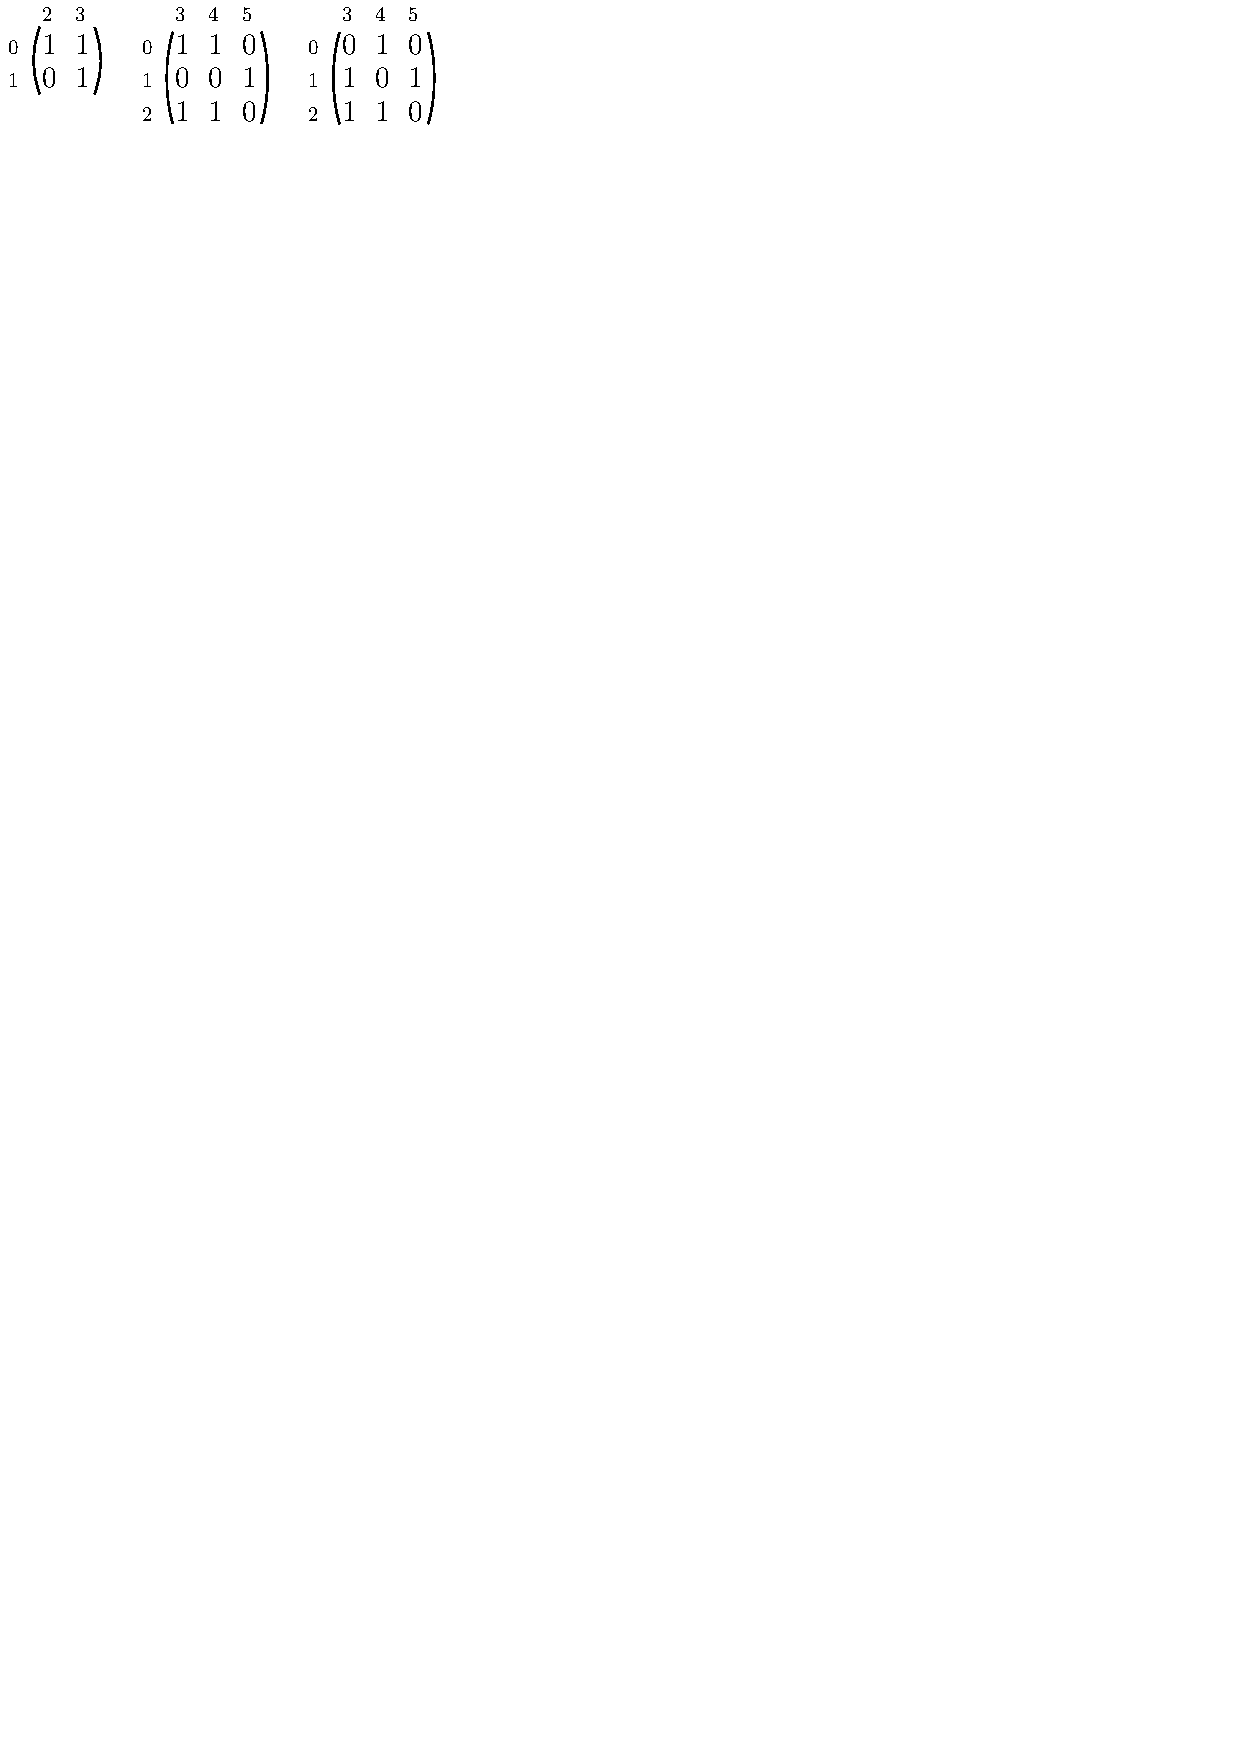
\includegraphics[width=100mm]{../img/avoiding.pdf}
\caption{Matrix $M_1$ contains the pattern $P$, because a mapping $\{(0,0),(1,2),(2,3),(3,4)\}$ satisfies all the conditions. On the other hand, matrix $M_2$ avoids $P$ as there is no such mapping.}
\label{avoiding}
\end{figure}
%\centerline{\mbox{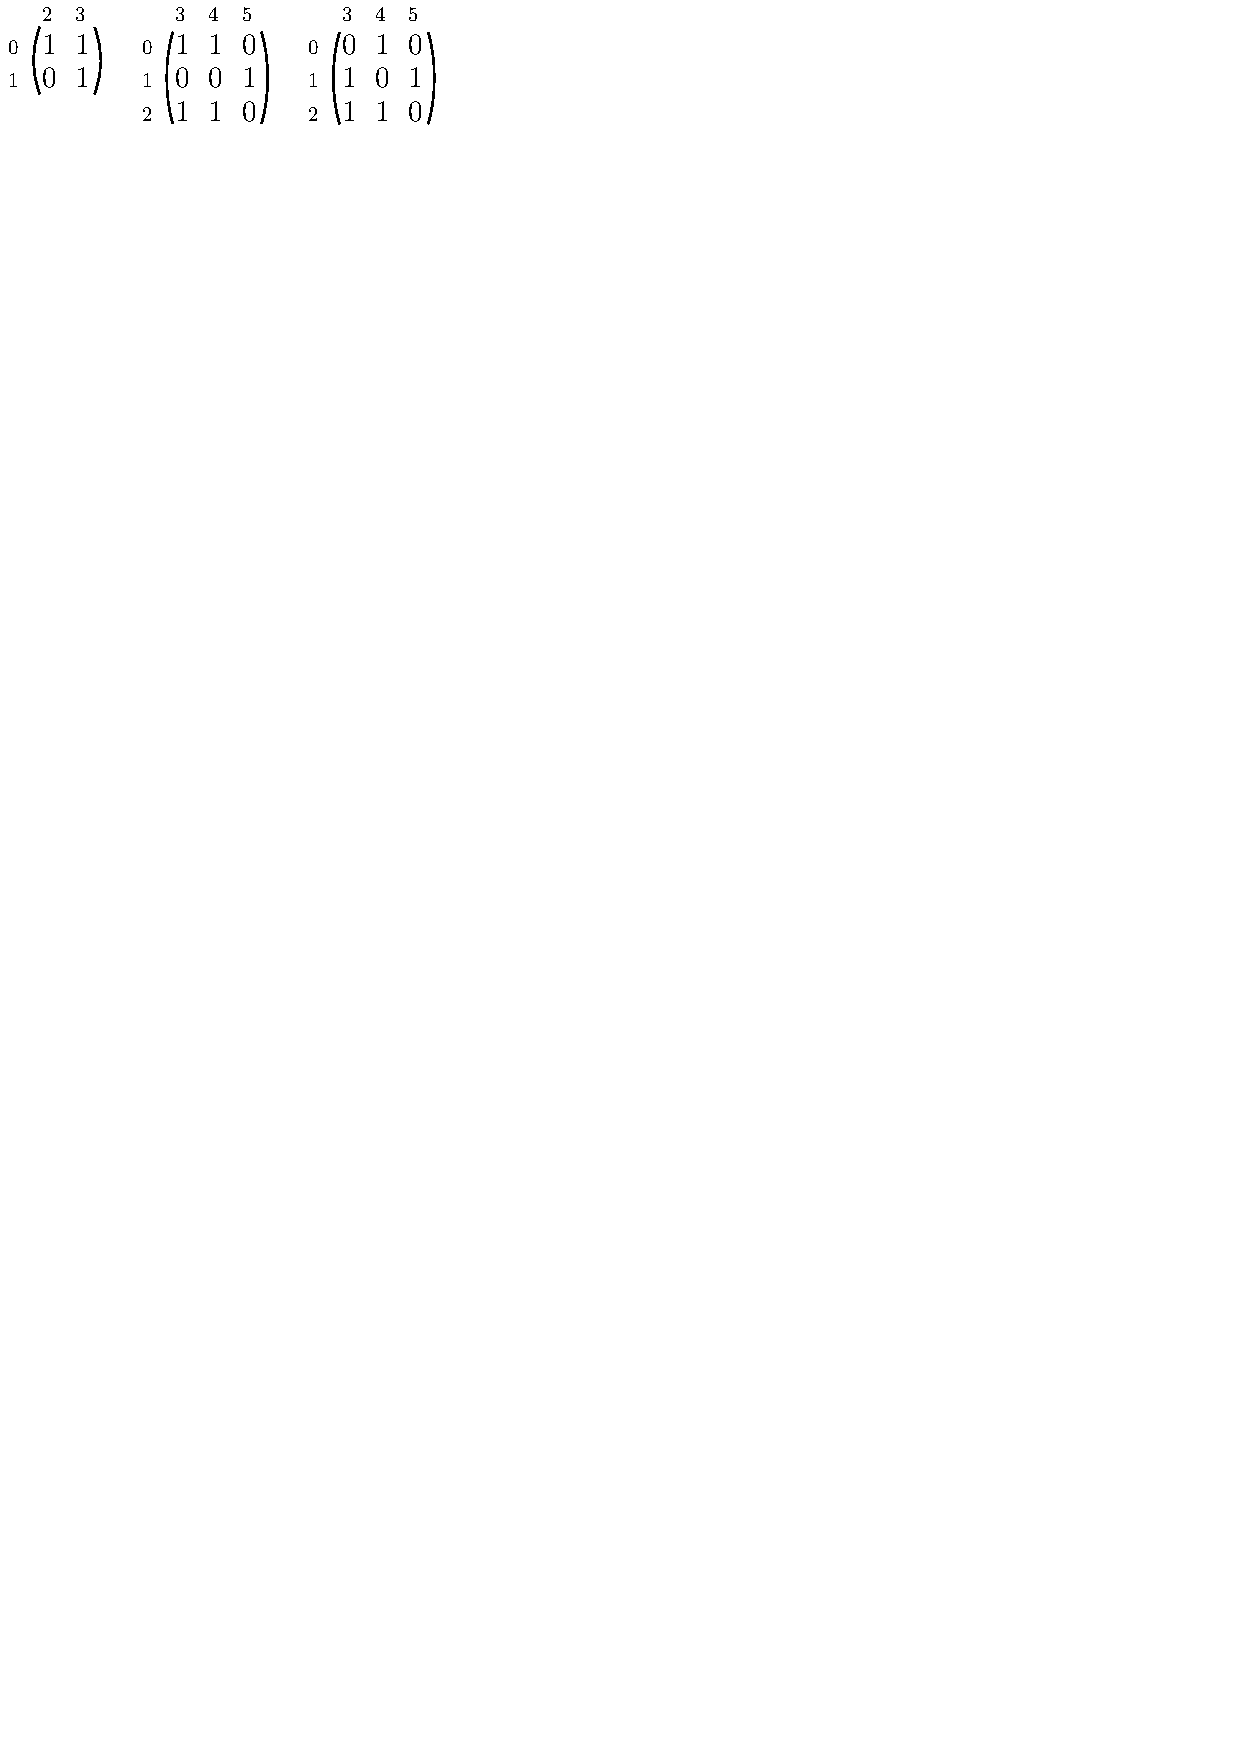
\includegraphics[width=100mm]{../img/avoiding.pdf}}}

The interesting cases are square matrices of size $n$ by $n$, where $n$ is big (going to infinity) and the size of a pattern (not necessarily square matrix) is small (constant). Even for a constant size forbidden pattern it is hard to determine the number of matrices of size $n$ that avoid it or to characterize, what properties they have. Sometimes we consider matrices avoiding more than just one forbidden pattern, in which case we denote the set of all forbidden matrices by $\mathcal{P}$. When a matrix avoids $\mathcal{P}$, it avoids every $P\in\mathcal{P}$. 
\begin{defn}
We denote by $\mathcal{M}_n(\mathcal{P})$ a set of all binary matrices of size $n$ by $n$ avoiding $\mathcal{P}$ as submatrices. We always call $M$ the square binary matrix for which we test the containing and $P$ the pattern (if there is one) that is being tested. Moreover, we denote by $h$ the height (the number of rows) of $P$ and $w$ its width.
\end{defn}
The area of pattern avoidance has been heavily studied for permutations and it also becomes more popular for their generalization - binary matrices. In most of the areas in combinatorics it is useful to explore properties of random objects and a lot of attention is directed towards random matrices when considering pattern avoidance. The goal of the work is, for given $n\in\mathbb{N}$ and set of forbidden patterns $\mathcal{P}$, to generate a uniformly random $M\in_R\mathcal{M}_n(\mathcal{P})$.
\subsection*{Generating random matrix}
One way to get $M\in_R\mathcal{M}_n(\mathcal{P})$ is to choose a matrix of required size completely at random, for such, test whether it avoids the pattern and simply repeat the process until we find one, which does. However, in the most interesting cases, only a small fraction of all matrices avoid the pattern and the process takes too long, to be practically useful.

For generating random permutations avoiding forbidden pattern, a different technique was introduced in \cite{MadrasLiu}. It uses a randomized process called Markov chain Monte Carlo, which we will abbreviate by MCMC. It is an iterative process, which for a well chosen Markov chain (more in \autoref{chap:mcmc}) approximates a random object. The algorithm by Madras and Liu was developed for permutations (permutation matrices) and it cannot be used for general matrices. In \autoref{sect:mmcmc} we show how to adapt the algorithm, which will lead us to a MCMC algorithm that approximates $M\in_R\mathcal{M}_n(\mathcal{P})$. To produce a good approximation the process needs to do a lot of iterations and despite the fact it is unknown what is the mixing time (the number of iterations required) of a MCMC process, in practice, the method does better than the trivial algorithm.
\subsection*{Testing avoidance}
In each step of our MCMC process we need to test whether a matrix avoids a pattern. We will show a very fast algorithm that only works for a special class of binary matrices (explained in \autoref{chap:walking}) together with a slightly less performing algorithm for a general pattern, which, again, comes as a generalization of an algorithm for permutations from the article by Madras and Liu and is described in \autoref{chap:general}.

In \autoref{chap:imp} we improve both our algorithms and introduce a parallel version of MCMC process, which further increases the performance of matrix generating.

In \autoref{chap:tdoc} some technical details are explained to make reading the code easier for reader and to describe user interface. The last chapter (\autoref{chap:udoc}) contains user documentation.
\addcontentsline{toc}{chapter}{Introduction}


\chapter{Markov chain Monte Carlo}
\label{chap:mcmc}
Our goal to generate $M\in_R\mathcal{M}(\mathcal{P})$ heavily depends on the theory of Markov chains. In this work we only define useful terms and state two important theorems. If you are interested in more details, see \cite{Madras}.

\section{Markov chains}
\begin{defn}
%We shall consider discrete-time \emph{Markov chain} $X_0,X_l,\dots$, where $X_i\in\mathcal{S}$, for a finite state space $\mathcal{S}$ and every $i$ (number of steps). The $k$-step transition probabilities are:
%$$p_{i,j}^{(k)}=Pr(X_{t+k}=j|X_t=i) \hspace{1cm} (i,j\in\mathcal{S})$$
Let $\mathcal{S}$ be a finite set of states and for every $i,j\in\mathcal{S}$ $p_{i,j}$ prescribed probability of a change of state from $i$ to $j$. Also let $X_0$ be a random variable with values from $\mathcal{S}$. We call a sequence $X_0,X_l,\dots$, where $X_i\in\mathcal{S}$ for every $i$ a \emph{Markov chain} if
$$Pr(X_{t+1}=j|X_t=i)=p_{i,j} \hspace{1cm} (i,j\in\mathcal{S})$$
\end{defn}
\begin{defn}
%A Markov chain is said to be \emph{symmetric} if $p_{i,j}^{(1)}=p_{j,i}^{(1)}$ for every pair of states $i$ and $j$.
A Markov chain is said to be \emph{symmetric} if $p_{i,j}=p_{j,i}$ for every pair of states $i$ and $j$.
\end{defn}
\begin{defn}
%A Markov chain is \emph{irreducible} if the chain can eventually get from each state to every other state, that is, for every $i,j\in\mathcal{S}$ there exists a $k\geq0$ (depending on $i$ and $j$) such that $p_{i,j}^{(k)}>0$.
A Markov chain is \emph{irreducible} if the chain can eventually get from each state to every other state, that is, for every $i,j\in\mathcal{S}$ there exists a $k\geq0$ (depending on $i$ and $j$) such that $Pr(X_k=j|X_0=i)>0$.
\end{defn}
\begin{defn}
%An irreducible chain has \emph{period} $D$ if $D$ is the greatest common divisor of $\{k\geq1|p_{i,i}^{(k)}>0\}$ for some $i\in\mathcal{S}$ (equivalently, for all $i\in S$). A chain is called \emph{aperiodic} if its period is 1. In particular, if an irreducible chain has $p_{i,i}^{(1)}>0$ for some $i$, then it is aperiodic.
If an irreducible chain has $p_{i,i}>0$ for some $i$, then it is \emph{aperiodic}.
\end{defn}
Let $p_{i,j}^{(k)}=Pr(X_{t+k}=j|X_t=i))$ denote the $k$-step transition probabilities for $k=0,1,\cdots$ and $i,j\in\mathcal{S}$. The transition probability matrix is $P=(p_{i,j})$.

Next we state two theorems allowing us to expect Markov chains to converge to a uniformly random state in $\mathcal{S}$ even if the initial state $X_0$ is not random. Both theorem can be found in \cite{Madras}.
\begin{thm}
Consider an aperiodic irreducible Markov chain with state space $\mathcal{S}$. For every $i,j\in S$, the limit $\lim_{k\rightarrow\infty}p_{i,j}^{(k)}$) exists and is independent of $i$; call it $\pi_j$. Furthermore, if $\mathcal{S}$ is finite, then
$$\sum\limits_{j\in\mathcal{S}}\pi_j=1\hspace{5mm}\wedge\hspace{5mm}\sum\limits_{i\in\mathcal{S}}\pi_ip_{i,j}^{(1)}=\pi_j$$
for every $j\in\mathcal{S}$. That is, if we write $\pi$ to denote the row vector whose entries are $\pi_i$, then $\pi P=\pi$.
\end{thm}
\begin{thm}
Suppose that an irreducible Markov chain on the finite state space $\mathcal{S}$ is symmetric. Then the equilibrium distribution is uniform on $\mathcal{S}$.
\end{thm}

\section{Markov chain for pattern-avoiding binary matrices}
\label{sect:mmcmc}
To generate a binary matrix $M\in\{0,1\}^{n\times n}$ avoiding patterns in $\mathcal{P}$, we create a Markov chain, whose states space is $\mathcal{M}_n(\mathcal{P})$. After sufficiently many iterations ($m$) of MCMC process we set $M:=X_m\in\mathcal{M}_n(\mathcal{P})$. We always begin with an initial matrix $X_0$ and the process looks like this:
\begin{enumerate}
\item For $i:=1,2,\cdots,m$:
\item \hspace{5mm} Set $X_{i}:=X_{i-1}$.
\item \hspace{5mm} Choose $r\in_R\{0,1,\cdots,n-1\}$ uniformly at random.
\item \hspace{5mm} Choose $c\in_R\{0,1,\cdots,n-1\}$ uniformly at random.
\item \hspace{5mm} Flip the bit at $X_{i}[r,c]$.
\item \hspace{5mm} If $X_{i}$ contains $\mathcal{P}$, flip the bit back.
\end{enumerate}

If the process starts with a matrix $X_0$ that avoids $\mathcal{P}$, then after every step it still avoids $\mathcal{P}$. Note that an iteration does not change the matrix if the condition 6 is satisfied. We need to show the Markov chain we presented meets all the conditions of both theorems:
\subsubsection{Symmetry}
Imagine a sequence of bits flipping that changes the $i$-th matrix to $j$-th one. The reversed order of the same sequence changes the $j$-th matrix to the $i$-th one.
\subsubsection{Irreducibility}
As the steps go, it is easy to see we can with non-zero probability create any matrix $M_1\in\mathcal{M}_n(\mathcal{P})$ from the zero matrix $0_n=0^{n\times n}$ by choosing the one-entries of $M_1$. When we can get from $0_n$ to $M_2$ by a sequence of flip changes, the reversed sequence is a sequence of steps from $M_2\in\mathcal{M}_n(\mathcal{P})$ to $0_n$. Thus, with non-zero probability we can always reach $M_2$ from $M_1$; therefore, the Markov chain is irreducible.
\subsubsection{Aperiodicity}
The Markov chain is irreducible so it suffices to show that there is an $i$ for which $p_{i,i}>0$. Clearly, there is a matrix for which there is at least one bit that cannot be flipped without creating a pattern (for example the one with the maximum number of one-entries) and this forces $p_{i,i}>0$.
\chapter{An algorithm for testing pattern-avoidance of a general pattern}
\label{chap:general}
In this chapter and Chapter \ref{chap:walking} we show algorithms for testing whether a pattern $P$ is contained in a square binary matrix $M$.

We begin with a very basic algorithm, which we then improve a lot to get a fast algorithm for testing the avoidance of a general pattern.

\section{Sketch of a brute force algorithm}
Let $L=(l_1,l_2,\cdots,l_{w+h})$ be a permutation of lines (rows and columns) of the pattern $P$ and $k\in[w+h]$. \emph{Partial mapping of level $k$} of lines of $P$ is a function $f$ from $L':=\{l_1,l_2,\cdots,l_k\}\subseteq L$ to lines of the big matrix $M$ satisfying three conditions: 
%The basic algorithm we use goes as follows. It takes a line $l$ (row or column) of the pattern and for each line $L$ of the big matrix it decides whether the pattern can be mapped there. It can, if three conditions are all met at once:
\begin{itemize}
%\item Both $l$ and $L$ are rows or they are both columns.
%\item If $l'$ is a line of $P$ parallel to $l$ that has been mapped previously to line $L'$, we want $l<l'\Leftrightarrow L<L'$. This means we want the mapped lines to be in the same order as they were in the pattern.
%\item If $l'$ is a line of the pattern orthogonal to $l$ that has been mapped previously to line $L'$ and there is a one-entry at the intersection of $l$ and $l'$, there has to be one-entry at the intersection of $L$ and $L'$.
\item Both $l'\in L'$ and $f(l')$ are rows or they are both columns.
\item If $l'\in L'$ and $l''\in L'$ are both rows or columns and $l'<l''$, then $f(l')<f(l'')$. This means partial mapping keeps the order of the lines.
\item If $l'\in L'$ is a row of $P$ and $l''\in L'$ is a column of $P$ and there is a one-entry at the intersection of $l'$ and $l''$, then there is a one-entry at the intersection of $f(l')$ and $f(l'')$.
\end{itemize}
The basic algorithm we use goes as follows. First it maps $l_1$ to all possible lines of $M$, creating partial mappings of $\{l_1\}\subseteq L$. For $k=2,\cdots,w+h$ it takes each partial mapping from the previous iteration and extends it by adding line $l_k$ to the partial mapping in all possible ways. If we manage to map all the lines of $P$, then $M$ does not avoid it and if at some point there are no partial mappings to extend it means $M$ avoids $P$.

The algorithm can be improved in two ways. Firstly, we can try to recognize unextendable partial mappings earlier than at the moment a line can no longer be mapped, for example by counting whether there is enough one-entries in between already mapped lines (more in Section \ref{sect:approaches}). Secondly, which is going to be fundamental for us, we can try not to remember more copies of different mappings that can be extended in the same way.

\section{Equivalent mappings}
There is no need to remember two different partial mappings of the same level if they can be both extended exactly the same way, because our function is only supposed to check whether a pattern can be mapped to a big matrix not to find all such mappings.
\begin{defn}
We call a line $l$ of a pattern $P$ \emph{important} for chosen permutation of lines of $P$, if one of the conditions is met:
\begin{itemize}
\item An adjacent line of the pattern has not been mapped yet.
\item There is a one-entry on the line $l$ at the intersection with line $l'$ that has not been mapped yet.
\end{itemize}.
Otherwise the line is \emph{unimportant} for the permutation.
\end{defn}
Whether a line is important or not only depends on the permutation, so if we have a line unimportant in a partial mapping of level $k$, it is unimportant in every partial mapping of level $k$.

At the beginning, when no line is mapped, all lines are important. After some lines get mapped, a line can become unimportant in the partial mapping as all lines that bound it are in the mapping as well. If a line is unimportant in a partial mapping of some level, it will stay unimportant in all extensions of the mapping we can find.
\begin{defn}
We say two partial mappings of the same level are \emph{equivalent} if all important lines in the mapping of that level are mapped to the same lines of the big matrix in both mappings.
\end{defn}
\begin{figure}[h!]
\centering
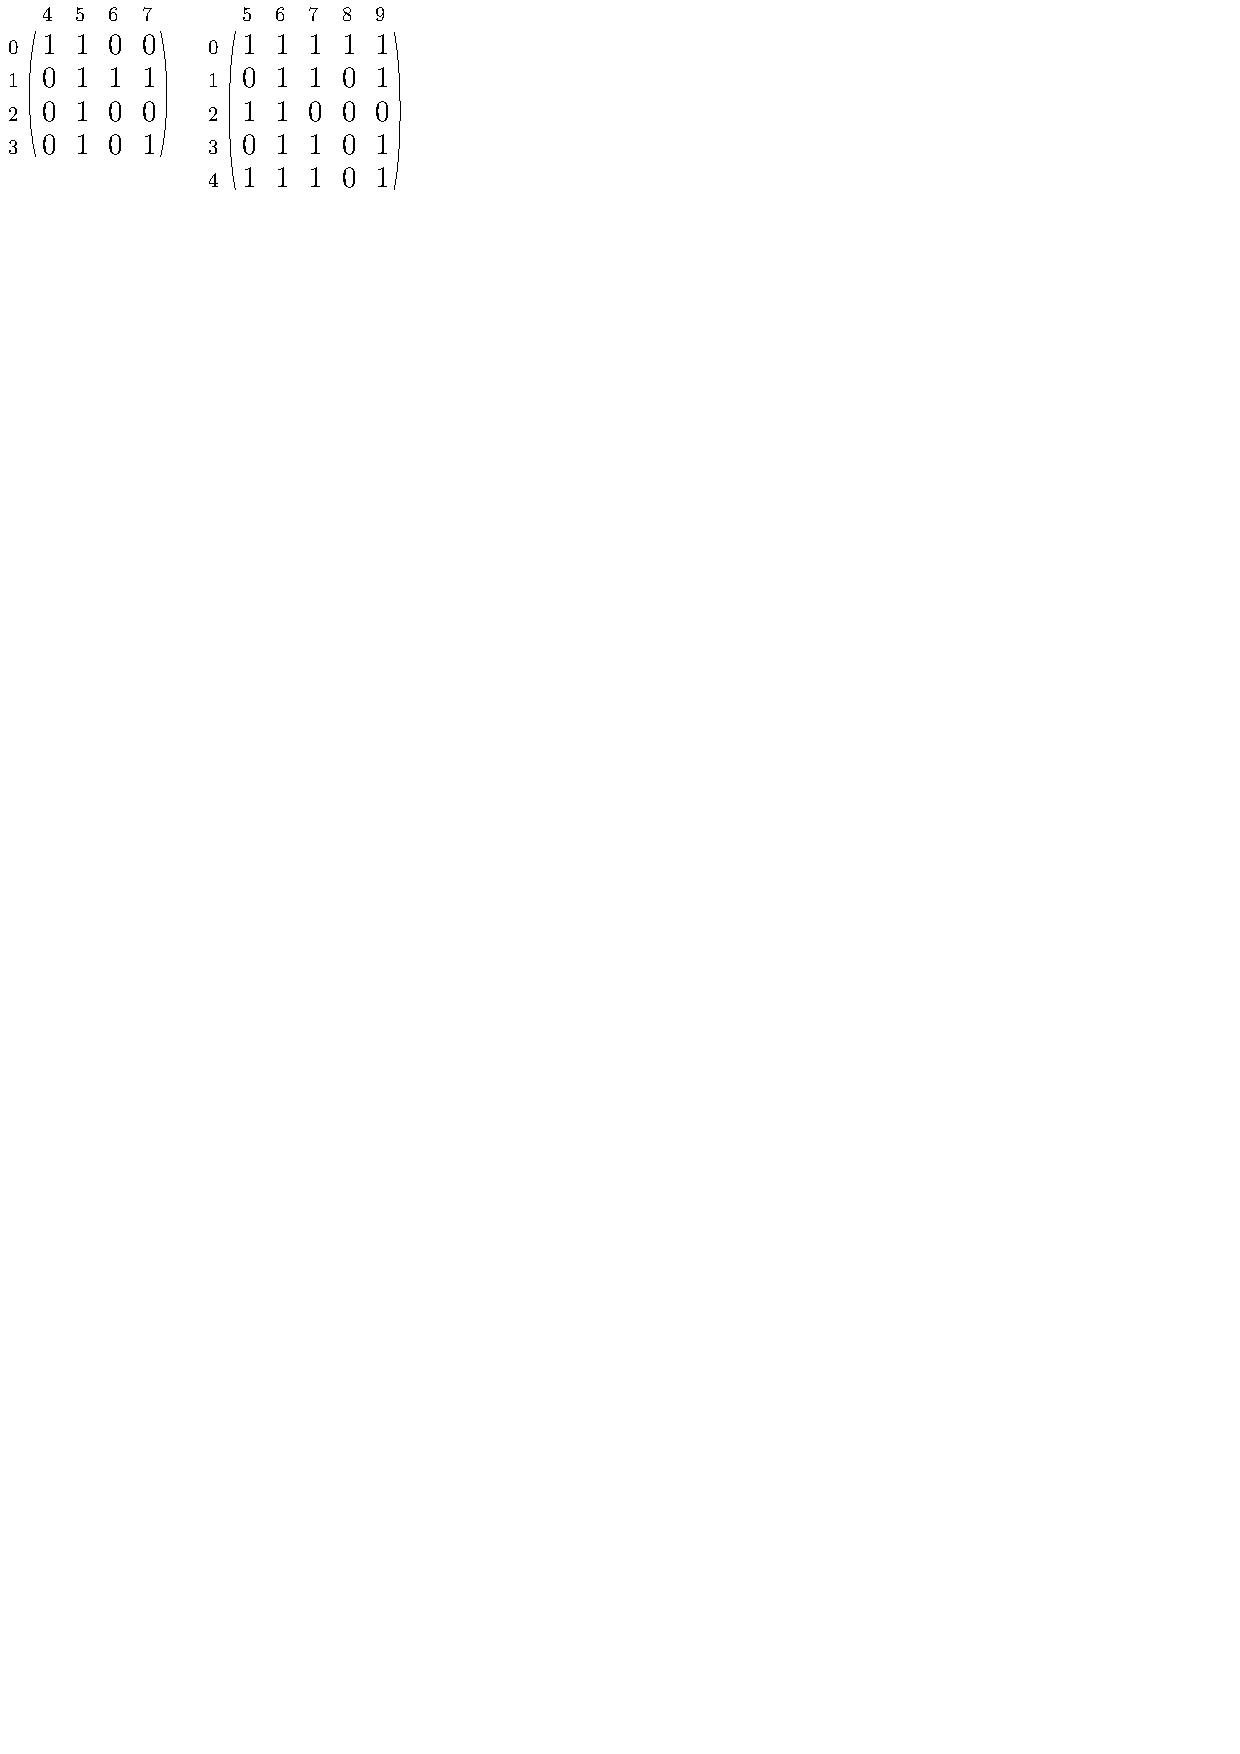
\includegraphics[width=100mm]{../img/equivalent.pdf}
\caption{An example showing unimportant line and equivalent mappings.}
\label{equivalent}
\end{figure}
%\centerline{\mbox{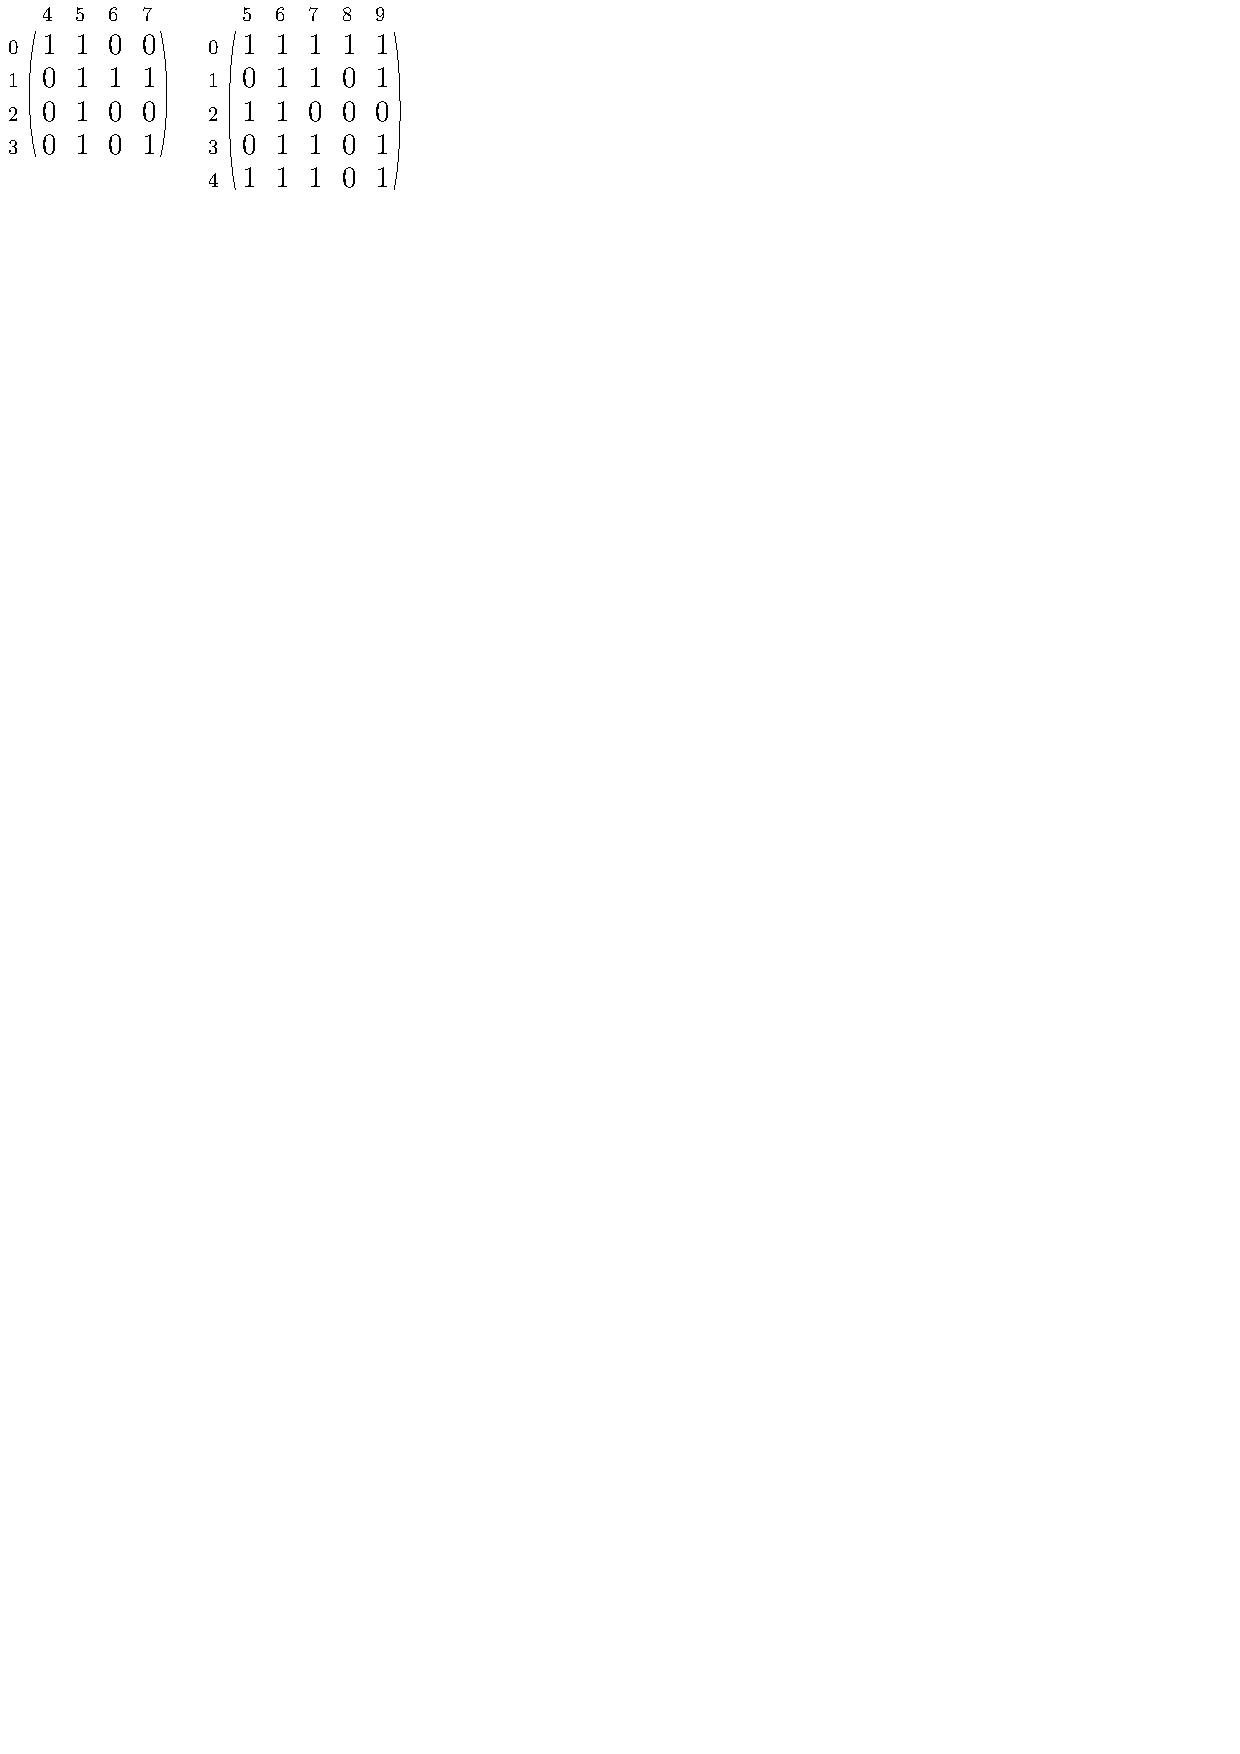
\includegraphics[width=100mm]{../img/equivalent.pdf}}}
For $P$ and $M$, binary matrices in Figure \ref{equivalent}, in partial mapping of level $4$ $f=\{(1,1),(2,2),(3,4),(5,6)\}$, line $2$ is unimportant because both lines $1$ and $3$ are mapped and so is line $5$ - the only line to intersect line $2$ in a one-entry. Line $3$ is important, because there is line $7$ intersecting it in one-entry, which is not mapped.

In the same situation as above, consider a different partial mapping $f'=\{(1,1),(2,3),(3,4),(5,6)\}$, which is a mapping of the same level as $f$ and only differs from $f$ in mapping line $2$. The line $2$ is unimportant and by the definition of equivalent partial mappings, $f$ and $f'$ are equivalent. The idea behind this notion is simple. It is not important where we map line $2$, because it does not restrict where we can map any other line that has not been mapped yet. This means that if a partial mapping $f$ can be somehow extended, the equivalent partial mapping $f'$ can be extended in the same way; therefore, it is sufficient to only extend one of them in order to find one full mapping. Note that it would be also sufficient to only extend one of the partial mappings if we were looking for all full mappings, but, in that case, we would need to keep the information about where the unimportant lines were mapped to.
\chapter{An algorithm for testing pattern-avoidance of a special pattern}
In the previous chapter, we have seen an algorithm for a general forbidden pattern which, using some heuristics, runs pretty fast. In this chapter, we introduce a special kind of a pattern, satisfying additional conditions, for which we can produce much faster algorithm.

\section{Walking pattern}
We call the specific pattern a walking pattern. The additional condition we want the pattern to satisfy is that there is a walk from one corner to the opposite one and all the one-entries of the pattern are contained on the walk.
\paragraph{Definition}
A \textbf{walk} in a matrix is a sequence of some of its entries beginning in the top left corner and ending in the bottom right one. If an entry at the position $[i,j]$ is in the sequence, the next one is either $[i+1,j]$ or $[i,j+1]$. Therefore, the length of an arbitrary walk is equal to $w+h-1$.
\begin{figure}[h!]
\centering
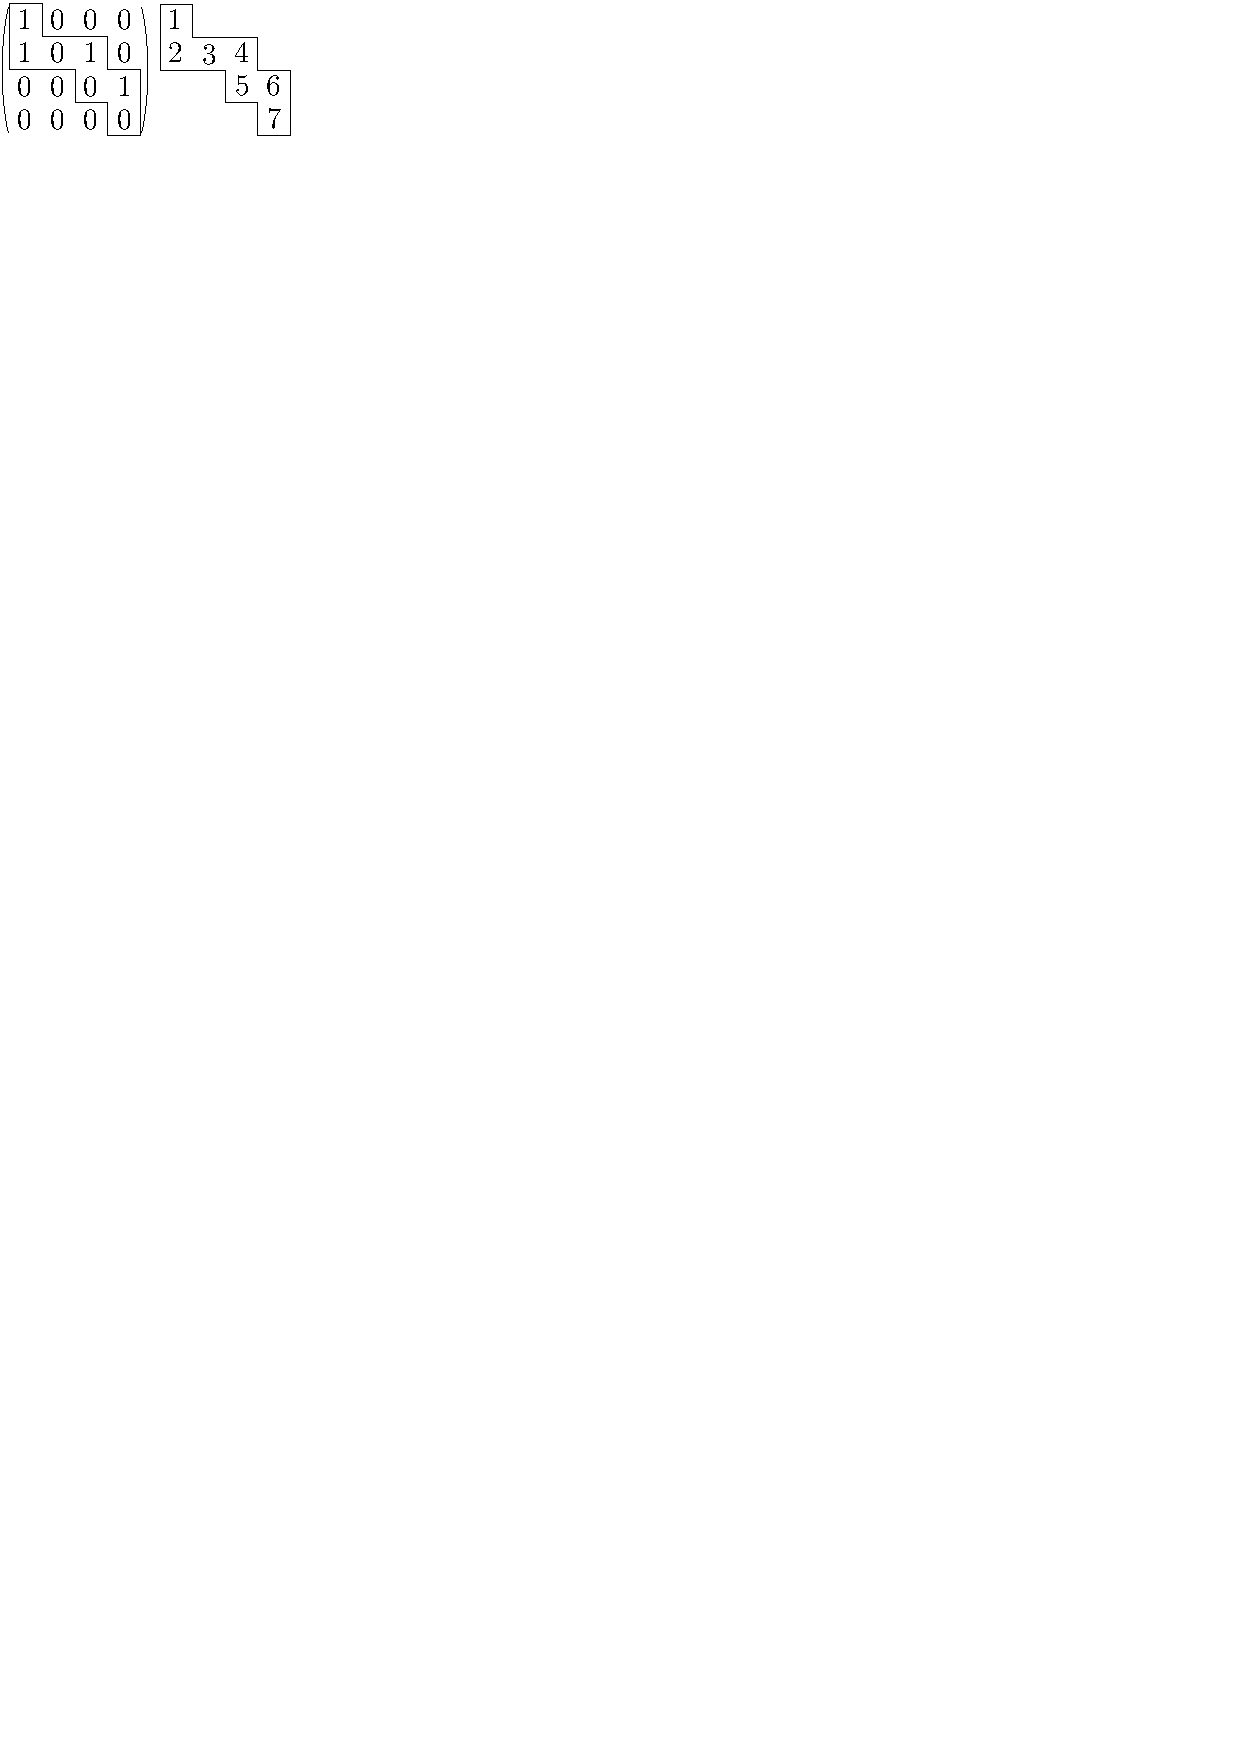
\includegraphics[width=100mm]{../img/walk.pdf}
\caption{An example of a walk and the order of its entries.}
\label{walk}
\end{figure}
%\centerline{\mbox{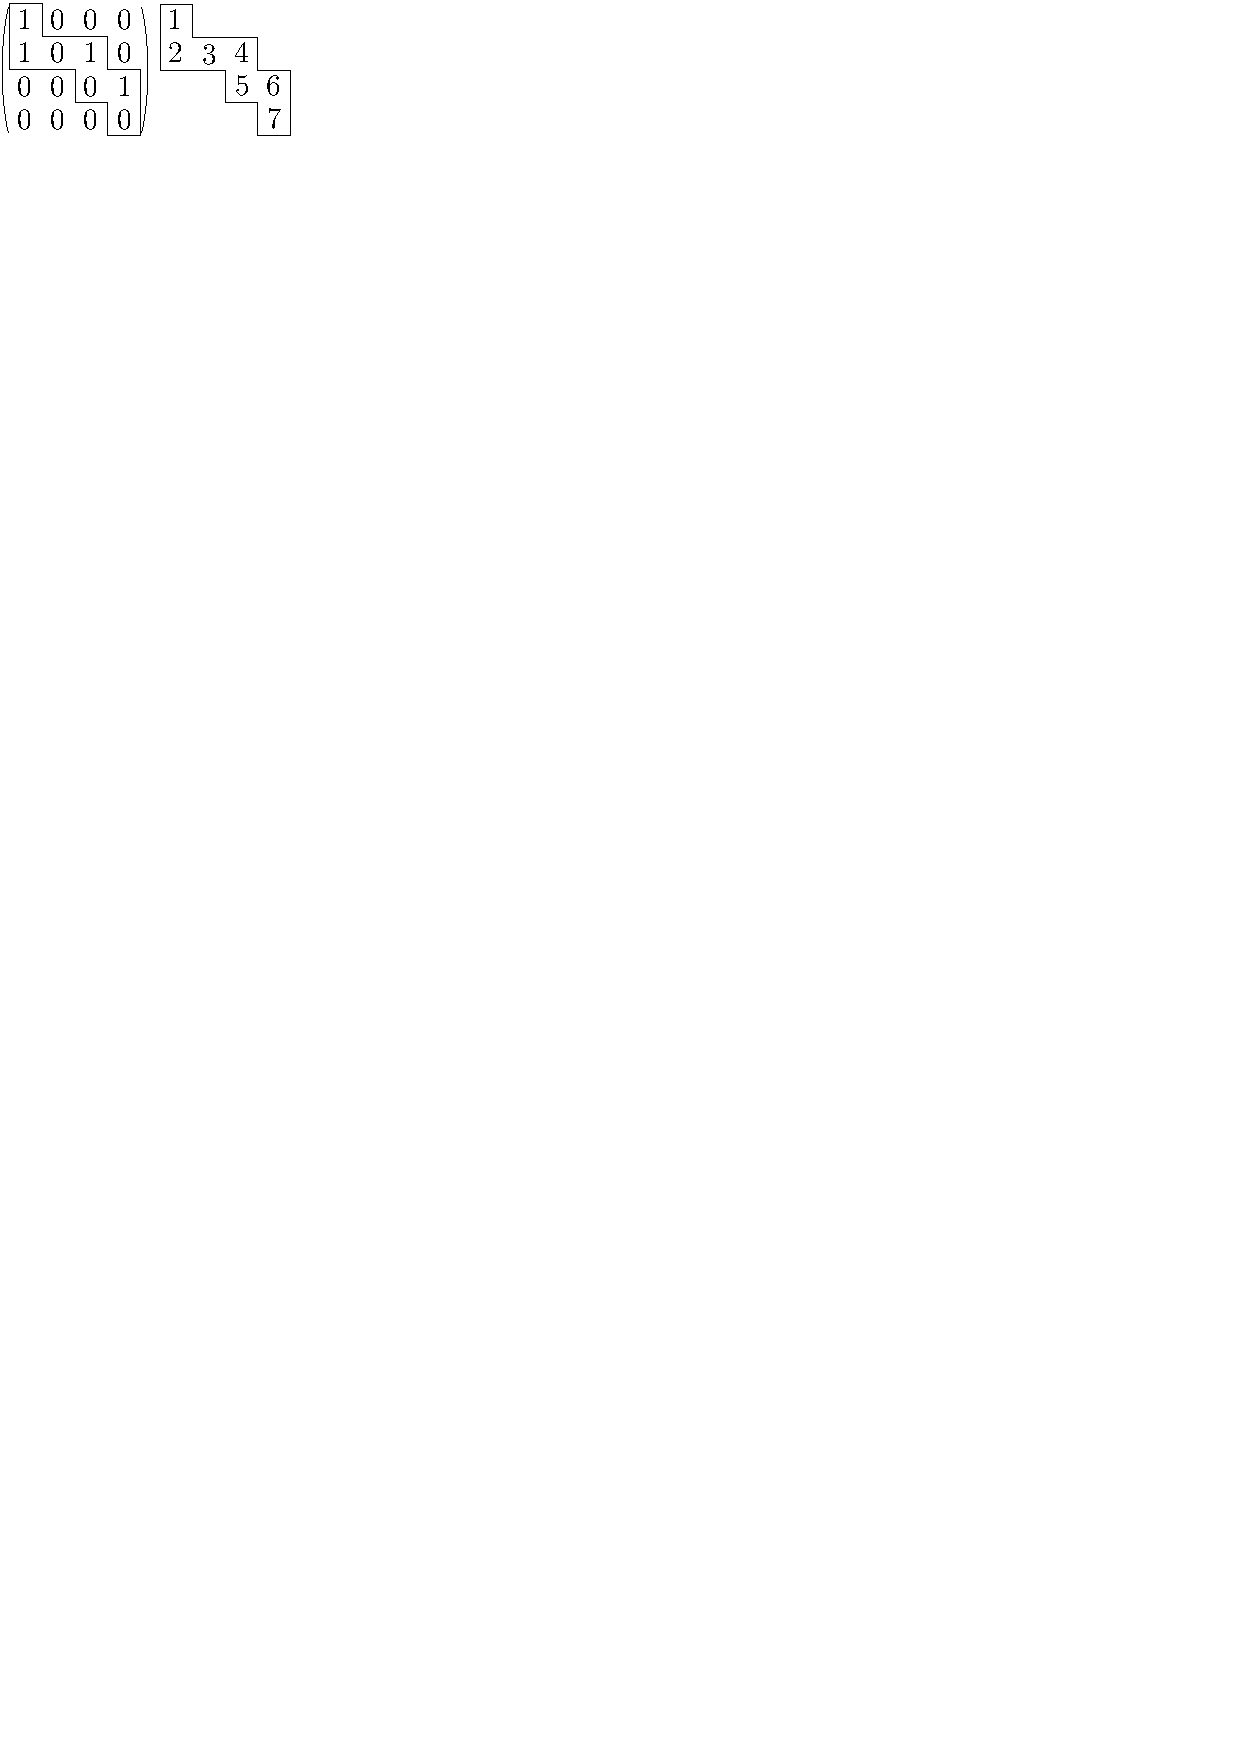
\includegraphics[width=75mm]{../img/walk.pdf}}}

In Figure \ref{walk} you can see a matrix that is a walking pattern as all the one-entries are included in a walk. Not all entries of a walk need to be one-entries though.

It can be shown a walking pattern with a walk is exactly a matrix avoiding a forbidden pattern
$$\left(\begin{array}{cc}
0 & 1 \\
1 & 0
\end{array}\right)$$

\section{Dynamic program}
Now that we know what walking pattern is, we show an algorithm deciding whether a pattern $P$ is contained in a big matrix $M$ or not.

The pattern $P$ is a walking pattern so there is a walk containing all the one-entries of the pattern. We choose one such walk arbitrarily and index its entries $e_1,e_2,\dots,e_{h+w-1}$ starting from the beginning of the walk. For each entry of the walk we remember whether its value is one or zero and whether the walk continues from the entry vertically, in which case we call it a \textbf{vertical entry} or horizontally, calling it a \textbf{horizontal entry}.

For an element $e$ of $M$ at the position $[i,j]$, the matrix $M_{\leq e}$ is a $(i+1)\times(j+1)$ submatrix of $M$ consisting of rows with the index smaller than or equal to $i$ and columns with the index smaller than or equal to $j$. The element $e$ then lies in the bottom right corner. Similarly, $M_{\geq e}$ is a $(n-i)\times(n-j)$ submatrix of $M$ consisting of rows with the index greater than or equal to $i$ and columns with index greater then or equal to $j$. The element $e$ is its first element.

To determine whether $P$ is contained in $M$ we find out for each element $e$ of $M$ what is the longest part of the pattern that can be found in $M_{\leq e}$. If there is an element for which we manage to find the last entry of the pattern, the pattern is contained in the matrix; otherwise, it is avoided.

For each element $e$ of $M$ at the position $[i,j]$ we remember two numbers. The number $c_v(e)$ says what is the longest part of the walk in $M_{\leq e}$ with the last entry in $j$-th column and being a vertical entry. The number $c_h(e)$, symmetrically, says what is the longest part of the walk in $M_{\leq e}$ with the last entry in $i$-th row and and being a horizontal entry.

An observation we make is that if we have a fixed element $e$ of $M$ and any other element $e'$ above $e$ in the same column then if $c_v(e')$ is equal to some $k$, then $c_v(e)$ is at least $k$. This means that for $e$ we can find the maximum part of the pattern ending in the column of $e$ and continuing vertically by looking only to elements in that column above $e$ and since this is true for all of them, it is sufficient to only check the value of the element right above $e$ (at the position $[i-1,j]$). Similarly the argument goes for the value of $c_h$ in horizontal way.

The algorithm iterates through diagonals. A diagonal in this matter of speaking is a subset of elements of $M$, such that all elements have the same sum of their coordinates. For example, zero diagonal only consists of an element $[0,0]$, the first diagonal contains elements $[0,1]$ and $[1,0]$, and so on.

For simplicity, in the pseudo-code below we do not deal with elements outside $M$ (like $-1,0$) explicitly. Instead for those elements we just assume the values of $c_v$ and $c_h$ are always equal to zero.

\subsection{The algorithm}
\begin{enumerate}
\item For $d=0,\cdots,w+h-1$
\item \hspace{5mm} For $e$ element of $d$-th diagonal at the position $[i,j]$
\item \hspace{1cm} $e_v:=[i-1,j]$
\item \hspace{1cm} $e_h:=[i,j-1]$
\item \hspace{1cm} $c_v(e):=c_v(e_v)$
\item \hspace{1cm} $c_h(e):=c_h(e_h)$
\item \hspace{1cm} If $w_{c_v(e)+1}$ can be mapped to $e$
\item \hspace{15mm} If $c_v(e)+1=w+h+1$
\item \hspace{2cm} Terminate - $M$ contains $P$ as a submatrix
\item \hspace{15mm} If $w_{c_v(e)+1}$ is a vertical entry
\item \hspace{2cm} $c_v(e):=c_v(e)+1$
\item \hspace{15mm} Else
\item \hspace{2cm} $c_h(e):=max\{c_h(e),c_v(e)+1\}$
\item \hspace{1cm} If $w_{c_h(e)+1}$ can be mapped to $e$
\item \hspace{15mm} If $c_h(e)+1=w+h+1$
\item \hspace{2cm} Terminate - $M$ contains $P$ as a submatrix
\item \hspace{15mm} If $w_{c_h(e)+1}$ is a vertical entry
\item \hspace{2cm} $c_v(e):=max\{c_v(e),c_h(e)+1\}$
\item \hspace{15mm} Else
\item \hspace{2cm} $c_h(e):=max\{c_h(e),c_h(e)+1\}$
\end{enumerate}

\centerline{\mbox{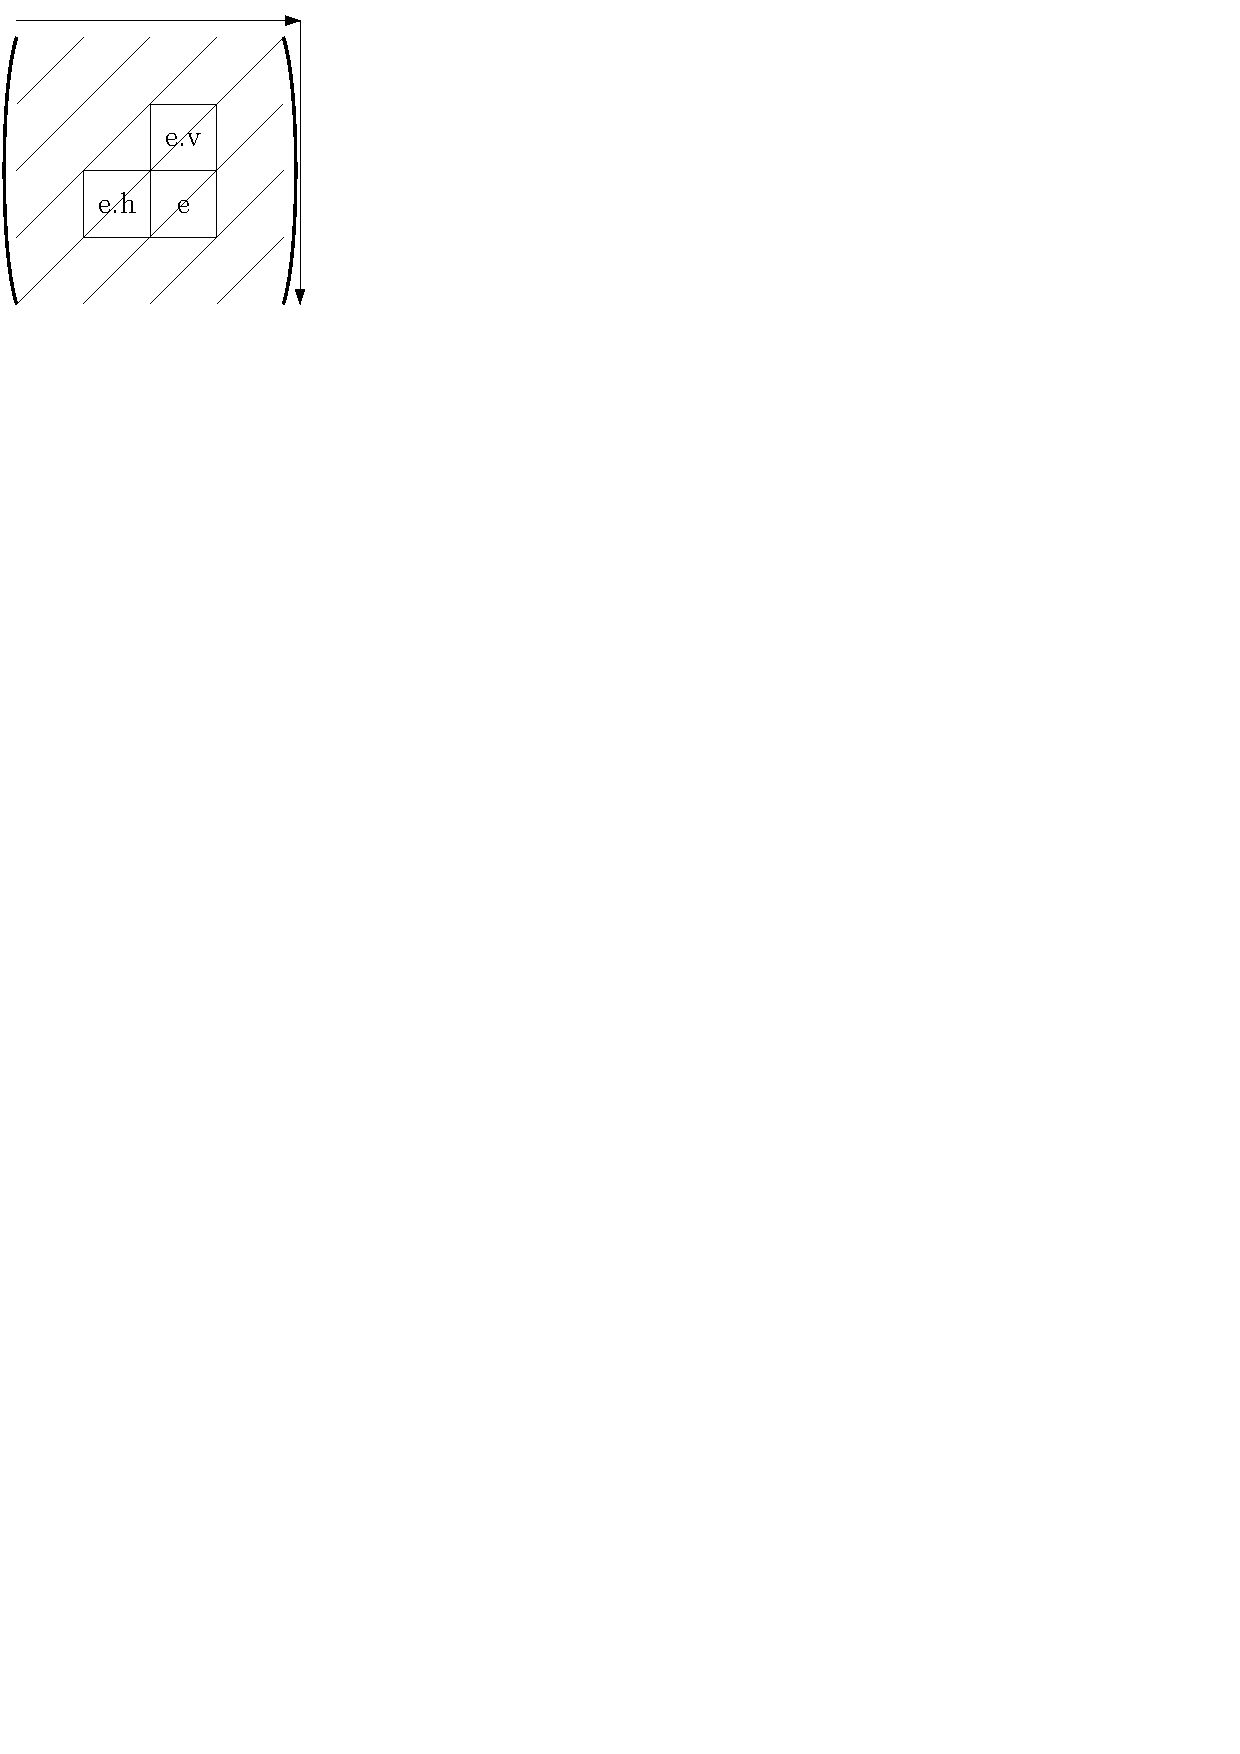
\includegraphics[width=60mm]{../img/walking_alg.pdf}}}

\subsection{Inner structure}
To run properly the algorithm needs two structures. The first one is a description of the walk, which is just an array of the values of its entries as well as the information whether the entry is vertical or horizontal. The second structure is a matrix of the values $c_v$ and $c_h$ as described above.

\subsection{Correctness}
We need to show that the values of $c_v$ and $c_h$ are always correct for the recomputed elements after at the end of the function. We proceed by induction.

For the first element it is definitely true since there can be only the first entry of the pattern mapped and we check just that.

When we compute an element $e$ of a computed diagonal $d$, by induction assumption all the diagonals $d'<d$ are correctly computed. In particular, the values are correct in the diagonal $d-1$. To compute the correct values of $e$, we use the values of two element on the diagonal $d-1$: $e_v$, which is right above $e$ and $e_h$, which is the first element to the left of $e$. If $e_v$ or $e_h$ are outside the matrix then from that direction we cannot expect to find anything more than just the first entry of the pattern and that is what we check for.

Let $v$ be the true length of the longest part of $P$ in $M_{\leq e}$ continuing vertically in the same column as $e$. Now if $e$ itself is not an entry of that part of the pattern, it is a different element $e'$ in the same column. But then the value of $c_v(e')$ is correctly computed by the inductive hypothesis and it is copied to all element underneath. Especially $e_v$ gets the value and the algorithm copies the value from it to $e$. On the other hand if $e$ is an entry of the part of the pattern we work with, it is the last entry. The entry right before the last one needs to be mapped to the same row or column; therefore, either $e_v$ or $e_h$ contain the part of the pattern shorter by one and the algorithm extends it to a correct value.

\subsection{Generalization}
The same algorithm, just rotated by 90 degrees, can be also used for a pattern where all one-entries are contained on a walk from top right corner to the bottom left one. Indeed the program uses it and if given a walking pattern it determines by itself which walk it is.

On the other hand a direct generalization for a general pattern does not work. While we can index all entries of the pattern, when trying to map a certain $w_k$ to an element it is not sufficient to just check whether $w_l$ is above and $w_l'$ to the left from the element.

\centerline{\mbox{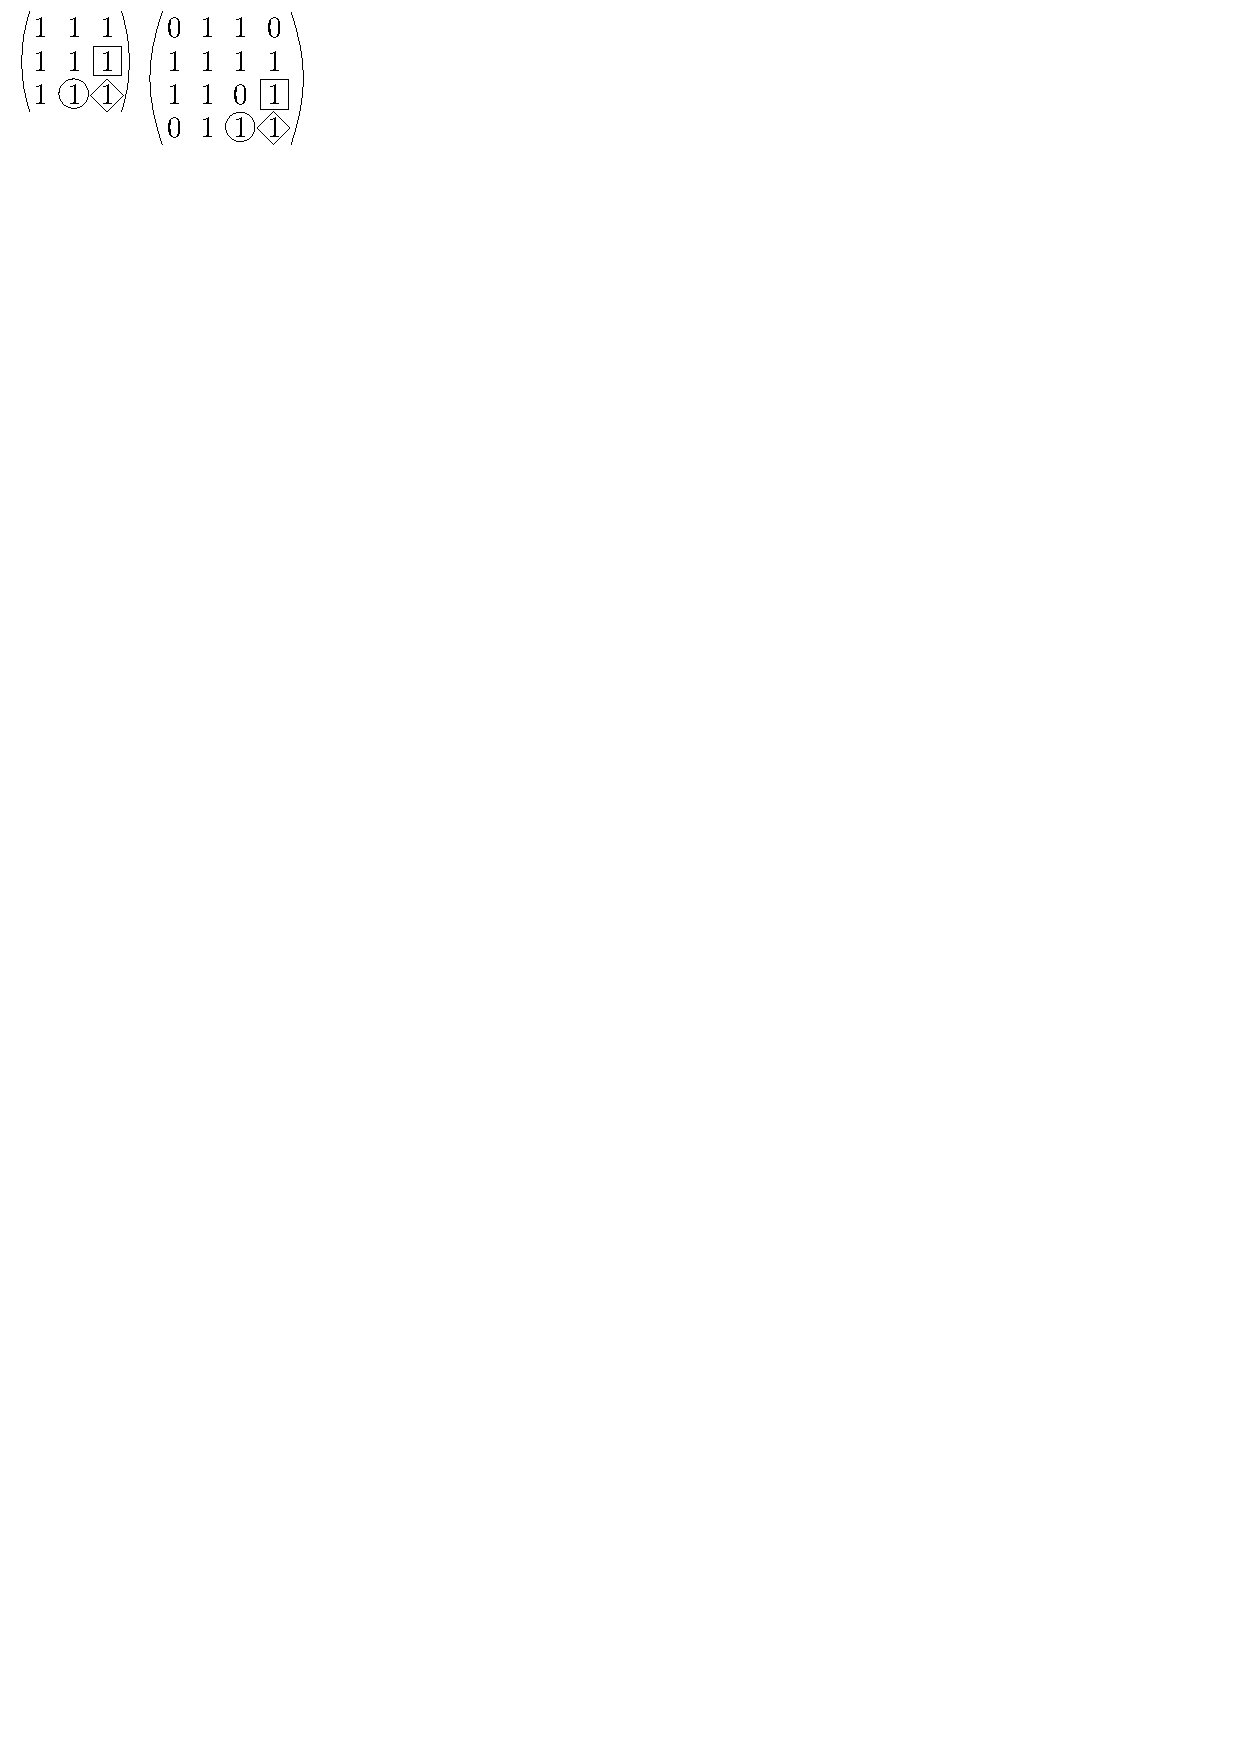
\includegraphics[width=75mm]{../img/nogeneral.pdf}}}

In the picture, let the matrix on the left side be the pattern $P$ and let $M$ be the other matrix. The entry in the square can be mapped to the element in the square and the same holds for entries in the circle but it is not a sufficient condition for the entry in the triangle to be mapped to the element in the triangle.
\chapter{Improvements to basic algorithms}
\label{chap:imp}
In this chapter we improve algorithms presented in previous chapters and introduce a parallel method of testing pattern avoidance.

\section{General pattern}
We start by improving the brute force algorithm from Chapter~\ref{chap:general}.

\subsection{Improving memory consumption}
The algorithm creates all possible partial mappings and checks whether at least one can be extended to a full mapping (mapping all lines of the pattern). To compute all the partial mappings of some level~$l$, it only uses mappings of level~$l-1$; therefore, it is enough to only store partial mappings of two levels in memory at any time.

In Chapter~\ref{chap:general} we also introduced the notion of (un)important lines and equivalence based on not using unimportant lines at all (they are fully bounded by other already mapped lines). When a line becomes unimportant, it stays unimportant till the end of the test; as a result, we can forget where we mapped those lines to save memory and only remember where we mapped important lines.

\subsection{Not mapping empty lines}
\begin{defn}
An \emph{empty} line is a row or a column that does not contain any one-entries.
\end{defn}
An empty line can be mapped to any line and we do not need to map it at all, as long as the algorithm does not map two lines surrounding an empty one to two consecutive lines.

\subsection{Using the last changed position}
The MCMC process always changes one element of the big matrix and asks whether it still avoids the pattern. If it does not and we know that before the change it did, we are sure the changed element $[r,c]$ is a part of the pattern. It is hard to use this fact in the algorithm. It just maps one line after another and we do not know at the beginning to which line the changed position lines should be mapped.

What we can do is to enforce that neither the~$r$-th line nor the~$n+c$-th one ($c$-th column) get skipped. We only look at the restriction for rows as the restrictions for columns are symmetrical. There are three situations we want to avoid:
\begin{itemize}
\item The first row of $P$ is mapped under the~$r$-th row. This prevents any other row to be mapped to the~$r$-th one and we do not want that.
\item The last row of $P$ is mapped above the~$r$-th row. This again prevents any other row to be mapped to the~$r$-th one.
\item Two adjacent rows $l,l+1$ of $P$ are mapped to $L<L'$ respectively and $L<r<L'$ which leaves no other row to be mapped to the~$r$-th one.
\end{itemize}

\subsection{Line order}
\label{sect:order}
An important thing, if we want the algorithm to run fast, is to choose a good line order. A line which is unimportant at level~$l$ in a line order may easily be important till the nearly last level in a different order.

We choose line order to hopefully enforce two things:
\begin{itemize}
\item Make as many unimportant lines as possible. This really allows the equivalence based improvements to kick in. The more lines are unimportant the more mappings become equivalent and the faster it is to iterate through all of them.
\item Recognize hopeless partial mappings as soon as possible. A partial mapping gets extended if the line does not break the rule that there is a one-entry where it needs to be. If we map all the rows first, the rule will get broken only after we start to map columns and we probably want to find out sooner.\\
\end{itemize}
In the program a user can either choose their own custom order or one of five algorithms with different main purposes:
\begin{itemize}
\item AUTO - this one tries the other three line orders and chooses the one which shows the best performance over some iterations on a matrix. While this may sound like a good thing to use, it is only so if an initial matrix is chosen and it takes a lot of time since a lot of iterations need to be made in order to make a good sample. I would recommend not to use AUTO order at all and instead to try all the line orders by hand with a number of iterations depending on the pattern and a good initial matrix; for instance, generated with a smaller number of iterations on the same pattern and with any line order.
\item DESC - the lines are ordered in descending order depending on the number of one-entries. This follows the idea to start with the lines that are the hardest to map. Note that this algorithm does poorly if there are a lot of lines with the same number of one-entries (for example an identity matrix).
\item MAX - it orders the lines so that the maximum number of important lines throughout the levels is as small as possible. This focuses straightforwardly to having many unimportant lines, which the program does not remember.
\item SUM - it orders the lines so that the sum of the numbers of the important lines is the smallest possible throughout all levels. The purpose is the same as in the MAX order and quite often it is the case both approaches produce the same order.
\item TWO - it orders the lines so that the maximum number of important lines in two consecutive levels throughout all the levels is as small as possible. This again focuses to having many unimportant lines, which the program does not remember. The constant two is chosen due to the fact general pattern always stores two levels of partial mapping at a time.
\end{itemize}

\subsection{Mapping approaches}
\label{sect:approaches}
The one thing the approaches we will introduce have in common is that they try to recognize those partial mappings that have no chance to be extended to a full mapping as early as possible.

While the algorithm introduced in Chapter \ref{chap:general} finds out the partial mapping is invalid only at the time it maps two lines having a one-entry at their intersection to two lines having a zero-entry at the intersection, different approaches try to reveal the fact we would end up in the situation earlier by checking more conditions.
\begin{figure}[h!]
\centering
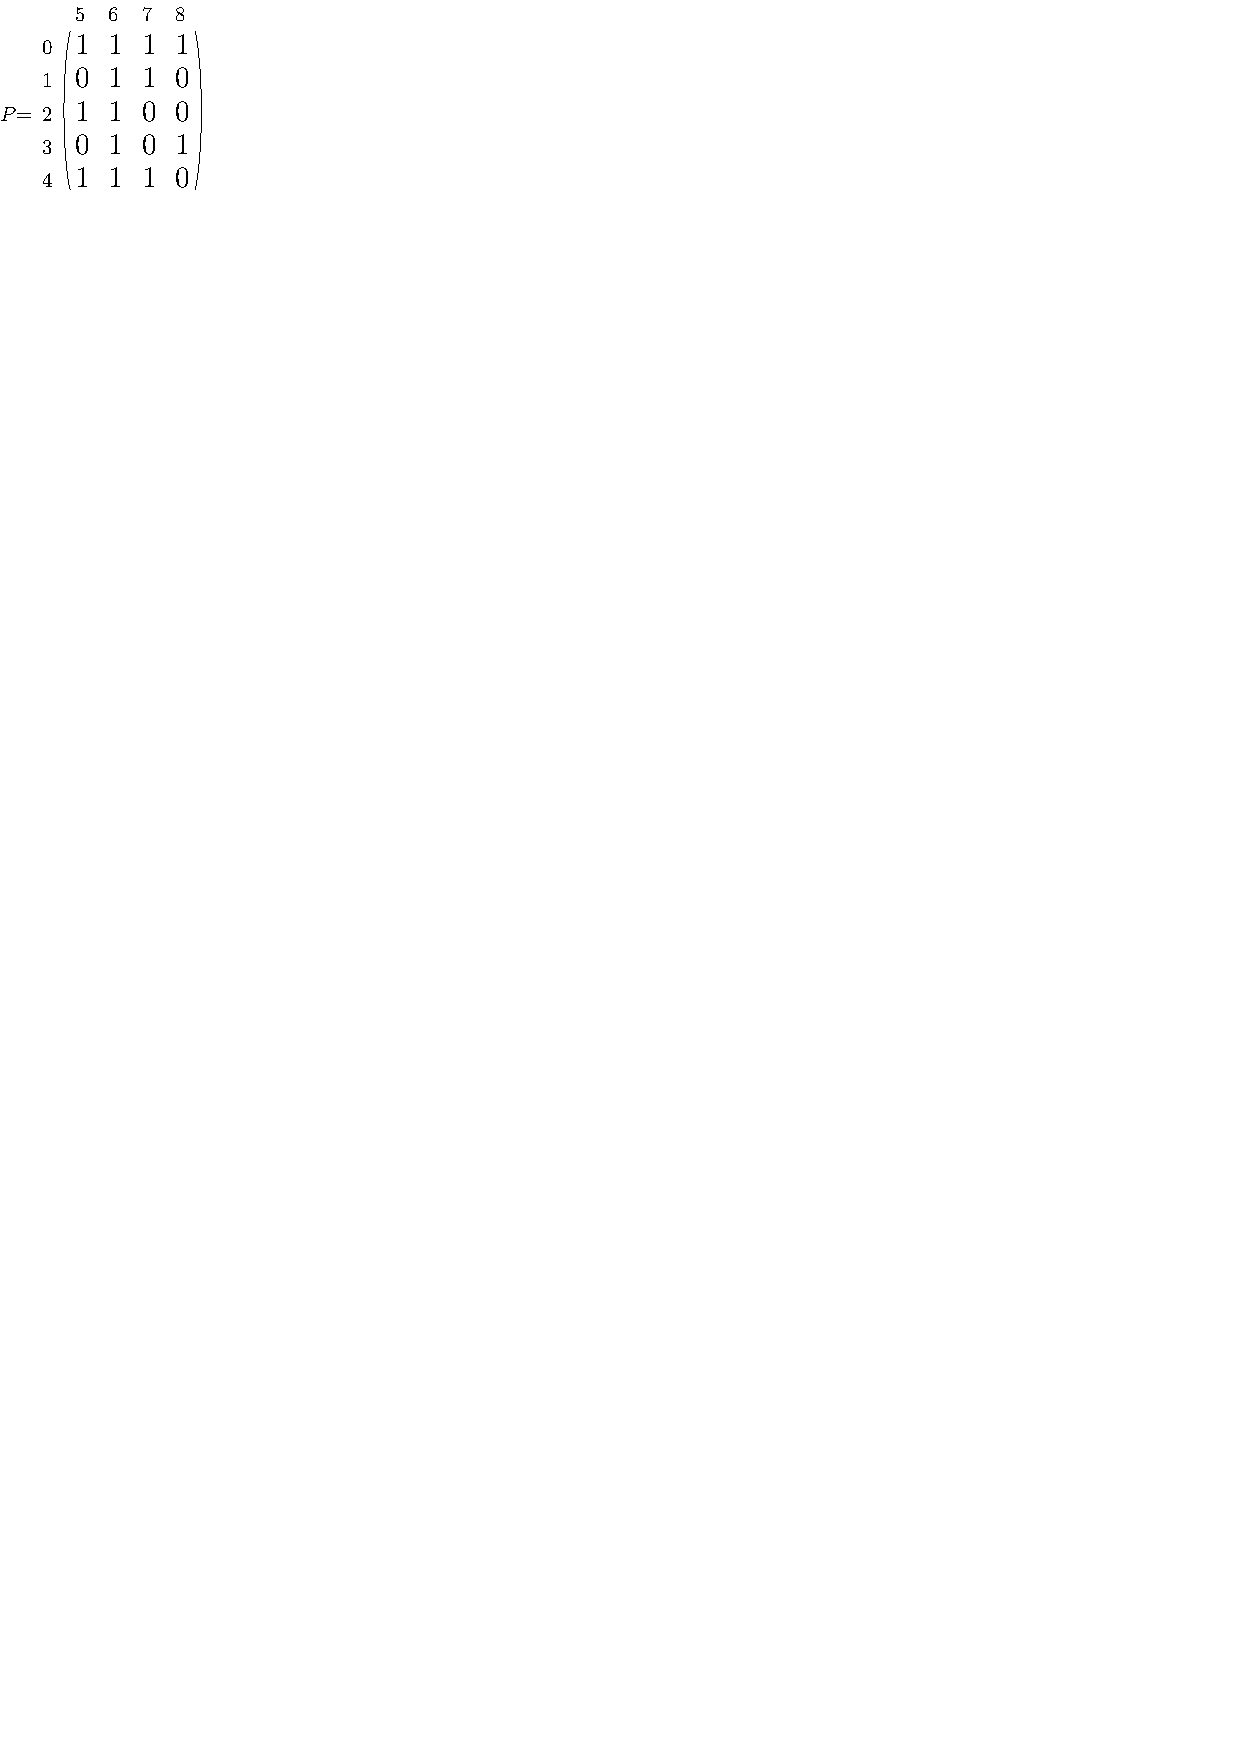
\includegraphics[width=50mm]{../img/approaches.pdf}
\caption{Pattern~$P$ on which we demonstrate mapping approaches.}
\label{approaches}
\end{figure}
Let $P$ from Figure~\ref{approaches} be the forbidden pattern and imagine a situation, in which only lines $0$, $3$ and $7$ are mapped and line~$6$ is currently being mapped. There are a few necessary conditions we can check:
\subsubsection{Enough one-entries}
\begin{figure}[h!]
\centering
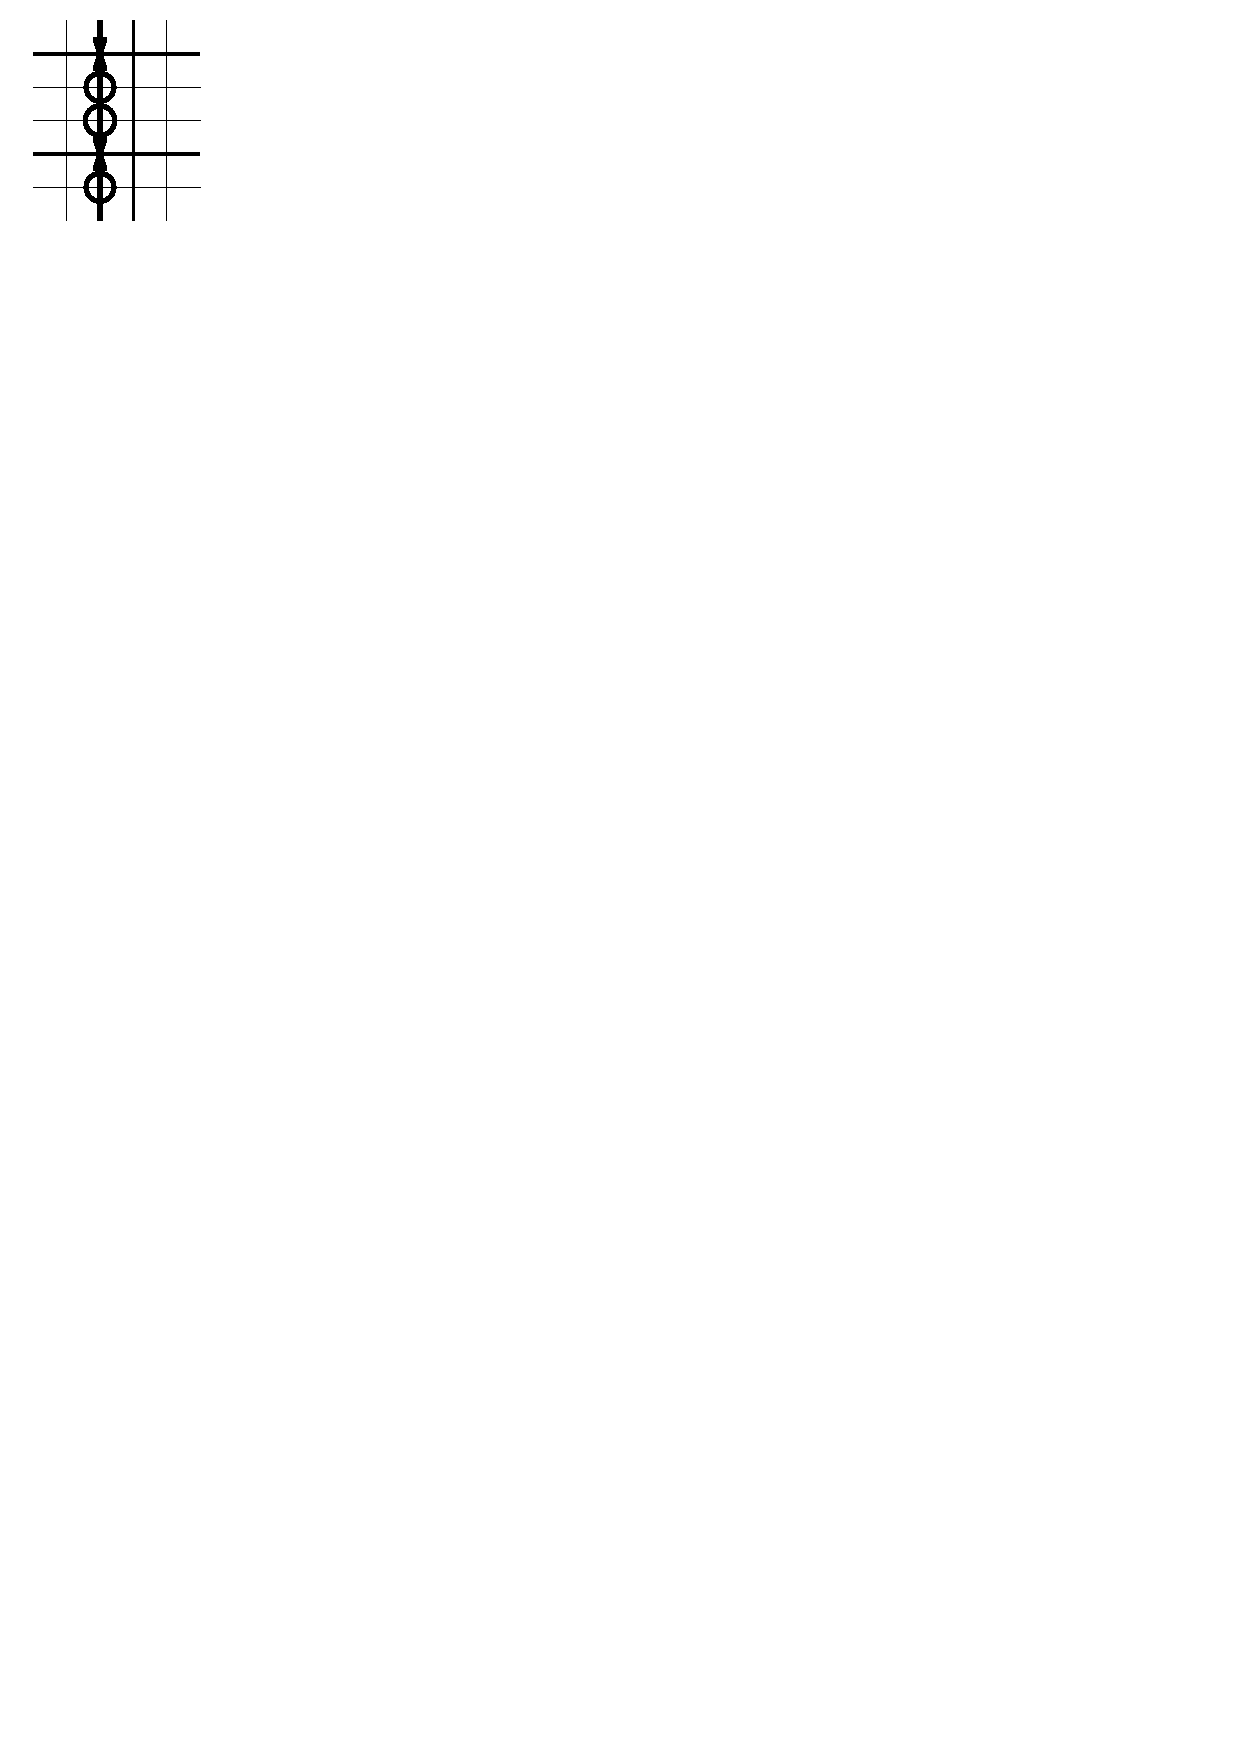
\includegraphics[width=55mm]{../img/enough_one-entries.pdf}
\caption{Checking whether there is enough one-entries. Bold lines in the picture are mapped and in circles are the positions where we look for one-entries.}
\label{enough}
\end{figure}
The first condition is that there are enough one-entries in between mapped lines, which is schematically shown in Figure~\ref{enough}. We check whether there is enough one-entries on lines in between those lines, where lines $0$ and $3$ are mapped, so that there is a hope we can map lines $1$ and $2$ there. Similarly, we check whether there is a one-entry below the line where line~$3$ is mapped so we can map line~$4$ there later.
\subsubsection{Recursive mapping}
\begin{figure}[h!]
\centering
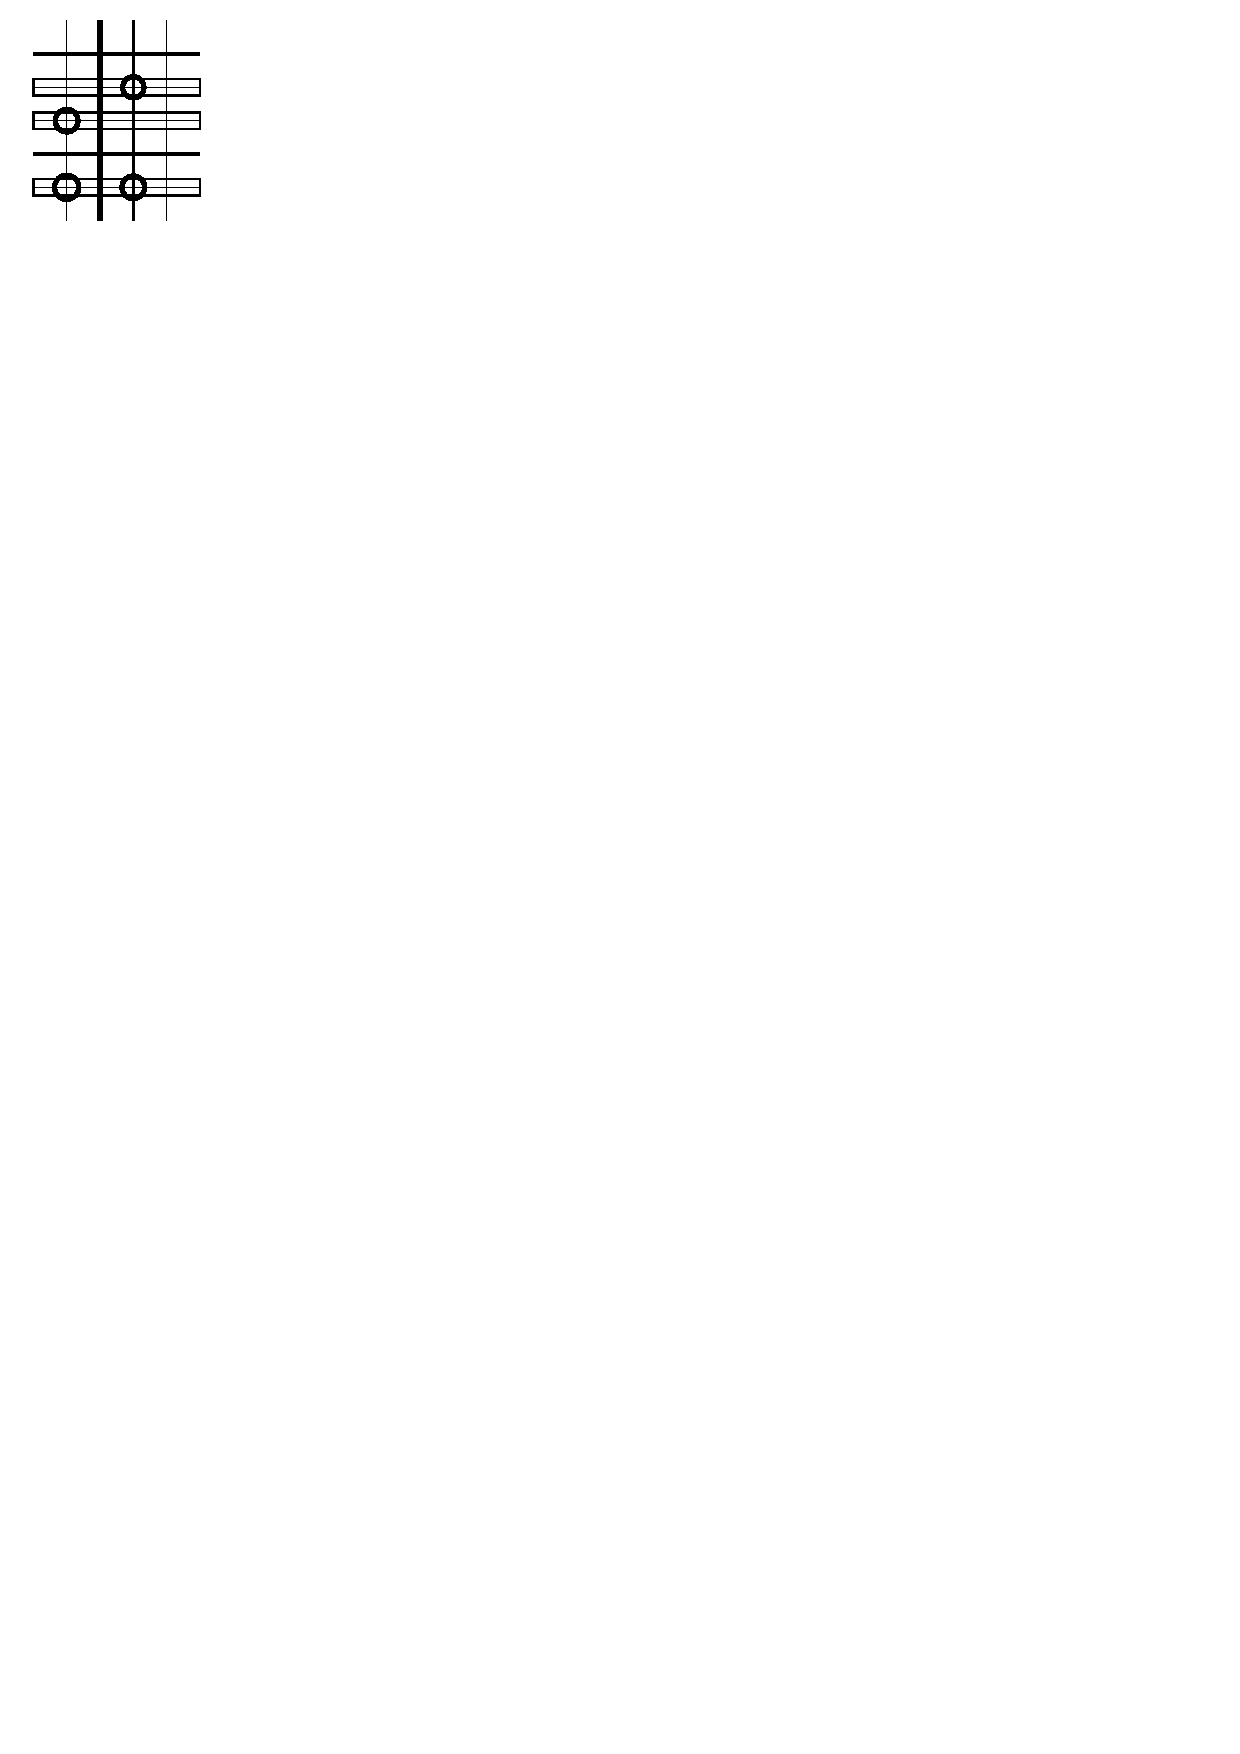
\includegraphics[width=55mm]{../img/recursive.pdf}
\caption{Checking whether crossed non-mapped lines can be mapped anywhere. Bold lines are mapped or being mapped, in rectangles are the lines we check and in circles are the positions where we look for one-entries.}
\label{recursive}
\end{figure}
While we were only testing whether there are enough one-entries in between already mapped lines in the previous approach, as you can see in Figure~\ref{recursive}, this time we also check whether those one-entries can be used for the lines that are intended to be mapped there. For example, when we check there is a one-entry to be used for line~$1$ later, we also check the line~$1$ can be mapped to the row with one-entry, which in this situation means to also check there is a one-entry at the intersection with the line to which the line~$7$ is mapped.
\subsubsection{Orthogonal bounds}
\begin{figure}[h!]
\centering
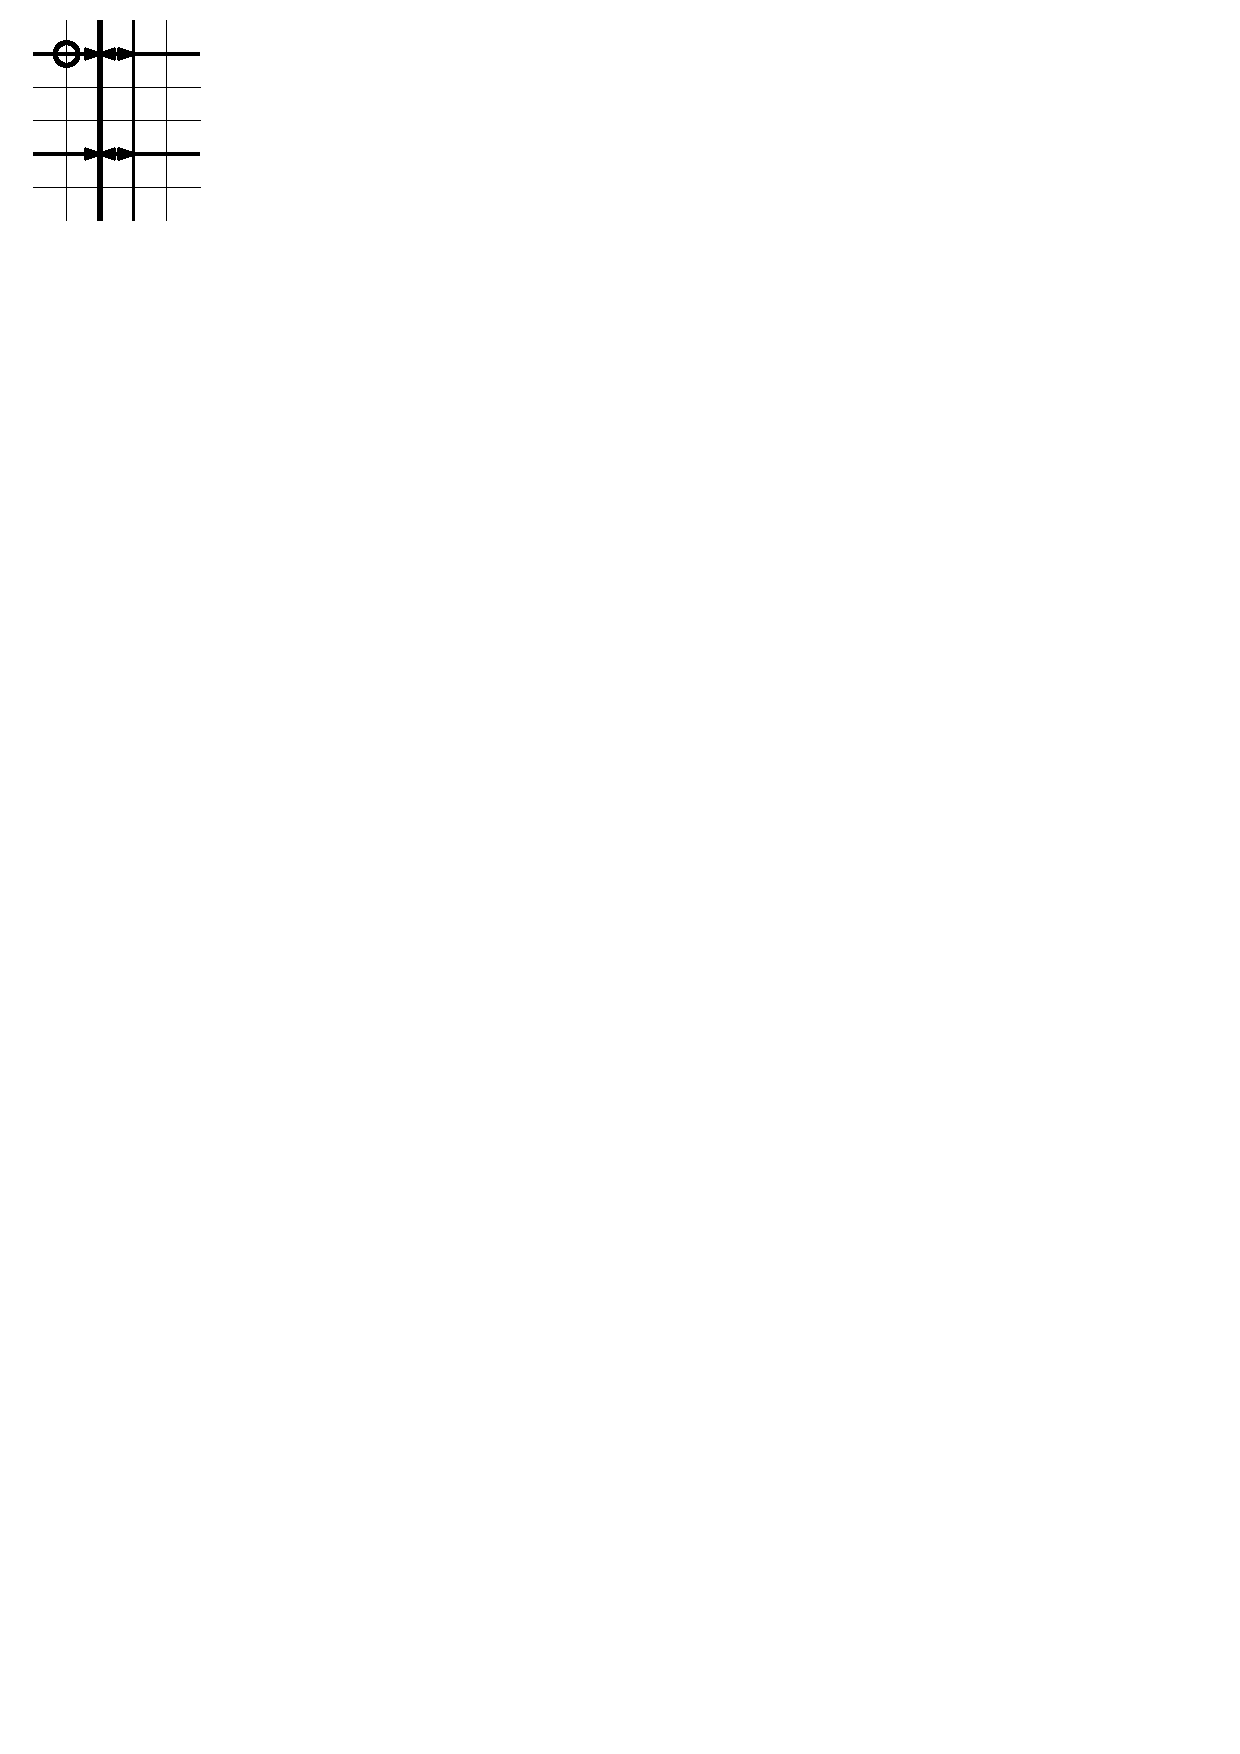
\includegraphics[width=55mm]{../img/orthogonal.pdf}
\caption{Checking whether there is enough one-entries on the orthogonal lines. Bold lines are mapped or being mapped and in circles are the positions where we look for one-entries.}
\label{orthogonal}
\end{figure}
As shown in Figure~\ref{orthogonal}, when we are adding line~$6$, we check whether there is enough one-entries on the already mapped lines orthogonal to line~$6$ between line~$6$ and the closest mapped lines next to line~$6$. The idea is same as in ``Enough one-entries'', but we check different lines.

\subsubsection{Usage}
These restrictions on the added lines are not a fixed part of the program. A user can decide which approaches they want to use in the configuration file.

When testing that was done for a fixed pattern, we found out it is useful to use all the mentioned restrictions when generating a matrix avoiding some patterns while it was much better not to use any of those restrictions for different pattern, which you can see in Table~\ref{approachestable}. For some patterns it also happened that using additional restrictions was useful for matrix of size $100\times100$ and for the same patterns it was better not to use them for generating a $500\times500$ matrix.
\begin{table}[]
\centering
\begin{tabular}{|ccc|c|r|c|c|c|r|r|}
\hline
\multicolumn{3}{|c|}{\textbf{Pattern}} & \textbf{n} & \textbf{\#iterations} & \textbf{one} & \textbf{rec} & \textbf{orth} & \textbf{time (sec)} & \textbf{memory} \\ \hline
1 & 0 & 0 & 100 & 100,000 & yes & yes & yes & 122.24 & 3,004 B \\ \cline{4-10} 
1 & 1 & 1 & 100 & 100,000 & no & no & no & 248.65 & 3,268 B \\ \cline{4-10} 
0 & 0 & 1 & 500 & 10,000 & yes & yes & yes & 1,072.53 & 5,380 B \\ \cline{4-10} 
  &   &   & 500 & 10,000 & no & no & no & 2,631.73 & 15,976 B \\ \hline
1 & 1 & 1 & 100 & 100,000 & yes & yes & yes & 1,512.56 & 3,268 B \\ \cline{4-10}
1 & 1 & 1 & 100 & 100,000 & no & no & no & 672.63 & 3,268 B \\ \cline{4-10} 
1 & 0 & 0 & 500 & 10,000 & yes & yes & yes & 10,276.60 & 9,128 B \\ \cline{4-10} 
  &   &   & 500 & 10,000 & no & no & no & 6,756.96 & 15,972 B \\ \hline
\end{tabular}
\caption{Testing additional restrictions of the generated matrix is useful in some cases but it comes with a performance drop in different cases.}
\label{approachestable}
\end{table}

\subsection{Using the whole structure in the next iteration}
\label{wholestructure}
It may seem like a good idea to store all the partial mappings. In the next iteration of MCMC, instead of finding all the partial mappings again, we only alter the mappings we remember. Let $i$ be the number of the iteration we are in, and $e$ be the element.

If the element~$e$ is changed from zero-entry to one-entry, for each partial mapping we have stored in previous iterations, we want to try to extend it only by the line that just changed. If we manage to extend a partial mapping, we then try to extend it to a full mapping in all possible ways (not only by using changed lines). When the new line in such a mapping becomes unimportant, we can stop looking for all possible extensions if the mapping is equivalent with a different one, which comes from previous iterations. This can be easily done by means already used in the standard algorithm.

However, if the element~$e$ gets changed from one-entry to zero-entry we need to go through the partial mappings and delete all those that use $e$. This complicates the algorithm as we can no longer forget unimportant lines. Moreover, for each partial mapping we need to remember how many partial mappings of the previous level can be extended to that one, to delete that mapping from the list if there are no longer any mappings extensible to it.

This can all be done, but it comes with three huge inconveniences:
\begin{itemize}
\item Memory consumption - there can be a lot of partial mappings and we need to remember them all. We need to remember mappings of all levels and while we can still use the equivalence when extending a mapping, we need to also store all equivalent mappings for the purposes of deleting.
\item The change from one-entry to zero-entry is no longer for free. If this change is done, we already know the pattern is not contained in $M$, but we still need to do a lot of work to change the structure in order to use it in the next iteration.
\item Reverting - if the change is unsuccessful (the pattern is contained) we need to revert the change which means to completely revert all changes we did to the list of partial mappings. This can be either done by making a backup copy of the whole structure and override the structure if needed, which again is very costly as the structure is huge, or we can remember what partial mappings are new (or deleted) and we go through all partial mappings and remove (add) those. This means to iterate through the big structure one more time for every unsuccessful change.
\end{itemize}
After realizing these issues it no longer looks useful to me and this version of the algorithm is not a part of the implementation.

\section{MCMC parallelism}
\label{sect:parallel}
To speed up computations, it is often possible to use parallelism. In this section, we show how to make the MCMC generator parallel, while still allowing both types of the pattern.

While the serial MCMC generator in each iteration changes one element in the generated matrix and checks whether it still avoids forbidden patterns, the parallel version makes several iterations at once, one on each copy of the generated matrix. This means that while iteration~$x$ is being computed by a thread, iteration~$x+1$ can at the same time be computed by a different thread. The issue is that the iteration $x+1$ does not know what is going to be the state of the generated matrix at the time it should start. It expects iteration~$x$ to fail - not change the generated matrix at all, counting on the fact, it is unlikely a change does not create a mapping of the pattern, and starts with the same matrix as iteration~$x$. If iteration~$x$ succeeds, then the computed iteration~$x+1$ is invalid and the iteration is going to be recomputed again, starting with the correct matrix.

When the parallel version of MCMC generator is chosen and it is assigned $n$ threads, it creates $n-1$ private copies of the generated matrix and $n-1$ private copies of patterns class. For $i=1,\dots,n-1$ it assigns $i$-th thread, called worker, to a pair of $i$-th copy of the matrix and $i$-th copy of patterns. The last thread, which we call the main thread and which has exclusive access to the master copy of the generated matrix, makes one change of a bit in each private copy of the matrix and makes the corresponding worker check the avoidance.

The job of a worker is only to check if its copy of the matrix still avoids the pattern when one bit is changed. On the other hand, all synchronization is left to the main thread. As mentioned before, one iteration of the MCMC process can be recomputed several times. We still want the generator to satisfy the conditions we have for the Markov chain (more in Section~\ref{sect:mmcmc}) in order to approximate a random matrix. To achieve that, if a computed iteration~$x$ succeeds (and changes the generated matrix), all the other computed iterations that would follow after the iteration~$x$ become invalid and they all have to be recomputed. The process ends when all iterations get computed.

For the sake of clarity, from now on, we will not be talking about iterations but about tasks. A task is basically one iteration of the MCMC process. The usefulness of this notation comes with an ID - a number, unique per task, assigned to each task, starting with $1$ and always increasing. For a pair of consecutive iterations $x$ and $x+1$ it will always be the case that if task~$a$ is the last task to compute iteration~$x$ (which means the iteration does not get recomputed ever again after) and task~$b$ is the last task to compute iteration~$x+1$, then the ID of $a$ is lower then the ID of $b$. Also there is no point, in which two different tasks would be computing the same iteration at the same time. If tasks with IDs $c<d$ computed the same iteration, it must have been the case an earlier iteration succeeded when task with ID~$c$ was computed and after it got removed, task with ID~$d$ was assigned to recompute.

At any point in time, we only consider those tasks, that are being computed or those that wait to be processed (not those that have been processed), which means the lowest ID of tasks we consider increases in time.

When a task ends and it has the lowest ID (we can always wait for the task with the lowest ID) we do:
\begin{itemize}
\item if it fails:
\begin{itemize}
\item Do nothing - there is no change to propagate to the master copy of the generated matrix and all the tasks with higher ID expected this task to fail, which it did.
\item This increases the lowest ID by exactly one, as the task we speak of got processed.
\end{itemize}
\item if it succeeds: 
\begin{itemize}
\item The main thread propagates the change tested by the task to the master copy of the generated matrix.
\item All the other tasks get removed as they all had a higher ID -- they computed iterations that follow after the one just computed and they expected the task to fail, which it did not.
\item This increases the lowest ID by more then one, because there are tasks that got removed and one that got processed.
\end{itemize}
\end{itemize}

\subsection{Example of the MCMC process for $n$ threads}
At first, iterations $1$ to $n-1$ are assigned one to each worker as tasks with ID $1$ to $n-1$ with the same order as the order of iterations. If iteration~$1$ is not successful (which all the other iterations count on), everything is alright. However, if the iteration (its task) is successful, all the results of other tasks (and some of them might have been already finished) are cleared and those iterations get recomputed in tasks $n$ to $2n-3$ and the worker that computed task with ID $1$ is assigned a new task with ID~$2n-2$ - to compute iteration~$n$. The result of the task gets propagated to the master copy of the generated matrix only if all the tasks $n$ to $2n-3$ fail, else is gets recomputed. This is what happens till the end.

\subsection{Speculative computing}
It may easily happen that a task not having the lowest ID ends first. In that case, we could just wait until it has the lowest ID and process it later. This is not a very efficient approach. Instead we process the task immediately, but we do not propagate the changes to the master copy of the generated matrix until all tasks with lower ID fail and we do not stop the workers processing tasks with lower ID. When a task succeeds we remove all the changes computed by tasks with higher ID and override their private copy of the generated matrix. Also it might happen a task with even lower ID succeeds as well. This leads to more and more overriding. Luckily this is the only precarious situation we may encounter and it can be dealt with, even without copying the possibly huge generated matrix.

The way we deal with these inconveniences is described in Chapter~\ref{chap:tdoc} and should be clear from the code (\cite{program}) itself.

\subsection{Reverting and synchronizing in the main thread}
The speculative computing discussed above is not the only improvement
we can make. It turns out to be costly to wake a thread to compute a trivial function, to set a few atomic variables and to fall asleep again. This happens a lot in the MCMC process. Every time a task succeeds it makes other workers revert the changes they computed and synchronize the successful change, which are both trivial functions.

To work around this problem we make a inelegant decision, which comes with very nice practical results. All the reverts and synchronizations are computed by the main thread instead of by an appropriate worker. There is no problem with concurrency because the worker is always asleep when a task is to be assigned and using the fact those tasks are really trivial, it does not make the rest of threads wait for the main thread for too long while it computes changes.
\pagebreak
\section{Walking pattern}
While the brute force implementation of an avoid algorithm for a general pattern was improved heavily, the algorithm for a walking pattern (see Chapter~\ref{chap:walking}) is very fast in its nature and cannot be improved. Or can it?

\subsection{Using the last changed position}
The MCMC process always changes one element~$e$ of the big matrix and asks whether it still avoids the pattern. If it does not and we know that before the change it did, we are sure $e$ is a part of the pattern (a one-entry of the pattern is mapped to it). Knowing that and using the same inductive proof as we did in the proof of correctness of the avoid algorithm (see Chapter~\ref{chap:general}) it is sufficient to only recompute the part of the inner structure (table of $c_v$ and $c_h$) under $e$ and check if the last entry of the pattern can be found there.

Not only that. We also know, using the fact the structure was completely correct before the change, that if the values of both $c_v$ and $c_h$ of an element did not change, the element will not cause the element underneath it to change and we no longer have to recompute other parts of the structure.

To use both these facts we replace the cycle through the diagonals by a simple queue, starting at the position of the last changed element and putting more positions in if the values of $c_v$ or $c_h$ are different than they were before recomputing. The function ends either when the pattern is discovered or when the queue becomes empty.

\subsection{Lazy implementation}
Lazy implementation of avoid and revert functions (see Section~\ref{patternapi}) is used when the MCMC parallelism (more in Section \ref{sect:parallel}) is chosen. While all the other types of patterns have a trivial implementation of revert function, when using the walking pattern, the inner structure needs to be modified even when reverting. The MCMC parallelism turned out to work much better if the revert calls are handled by the main thread and it requires the function to run as fast as possible so the other threads are not blocked by the call for too long. That is a reason why functions lazy revert and lazy avoid were created. A different, but not less significant reason is that because of concurrency, usually there are several revert calls after one avoid call; therefore, it is better to improve revert calls even with a downside of making avoid calls slightly slower.

The avoid function expects the inner structure of the walking pattern to be in a valid state and that requires some effort. To make lazy revert as fast as possible, we postpone the work until the next call of lazy avoid, meaning that lazy avoid then needs to do more things at once. It is no longer sufficient to only compute the submatrix under the position changed last as we did above, but it is necessary to also compute changes in the positions changed in those lazy revert calls that are postponed.

We discuss several approaches, starting with the simplest one and ending with the one that is fast and used in the final implementation.

\subsubsection{Recompute the whole structure every time}
The easiest way to implement lazy avoid is to always recompute the whole inner structure. In that case, we do not worry which positions are correct and which are not, because every time we find the pattern, we recomputed all the entries that form it, so we know it really is there.

The weakness is efficiency. If the whole structure was correct and there was a change of the last entry of the matrix it is sufficient to only recompute that one entry. Instead we recompute a possibly very big structure. This results in a very bad performance negating the advantage of parallel computation.
\subsubsection{Recompute only a part of the structure diagonal by diagonal}
A simple improvement is to remember the changes done in previous calls of lazy revert and together with the change done in lazy avoid call only recompute the part of the structure that has possibly changed.

This gets more complicated when an avoid call in the lazy implementation discovers the pattern in $M_{\leq e}$, because the avoid call returns as soon as the pattern is discovered, without recomputing the whole inner structure. It is still possible to remember some horizontal, vertical and diagonal bounds and use them to restrict the recomputed part of the matrix. However, the improvement is not that significant and we can do better.
\subsubsection{Queue of positions to recompute}
A different approach is closer to the one used in a standard avoid function. Instead of going through diagonals one after another, we have a queue of entries-to-recompute. It is no longer sufficient to have a standard queue since in different calls of lazy revert/avoid we can possibly change an entry of different priority (the smaller diagonal the more important) so we need to have some kind of a priority queue. That is exactly what I tried.

Using std::priority\_queue, the function has no more problems with recomputing the entries that were not influenced by the changes and uses all the benefits mentioned in the previous section. But the container does not come for free and in the end it turns out the price we pay for the operations on the priority queue make the whole implementation comparably slow as in the previous attempts.
\subsubsection{Two leveled queue of positions to recompute}
The final solution comes with the same idea, but a different storage. As the priority depends upon a diagonal (two entries on the same diagonal can be recomputed in any order) we only remember a priority queue of diagonals and an array of diagonals saying whether a diagonal is already a member of the priority queue. As far as the entries are concerned, for every diagonal we have a std::vector of entries-to-recompute as well as an array saying whether an entry is already a member of the vector. Finally, it is the case that the storage used is not only good theoretically but as the numbers say, also practically.

\section{Comparison of all methods}
We have improved all algorithms and added a parallel version of the MCMC process. The question is, whether our improvements were useful in terms of performance and memory consuming. I have done a few tests and in Table~\ref{measurements1}, Table~\ref{measurements2} and Table~\ref{measurements3}, you can see that at least in some cases walking pattern does much better than general pattern and that parallel computation was not added without a good reason. We always generate a matrix of size $n\times n$ and if there is one thread, we use the serial variant of MCMC process; otherwise, we use the parallel one.
\begin{table}[]
\centering
\begin{tabular}{|ccc|c|r|c|c|r|r|}
\hline
\multicolumn{3}{|c|}{\textbf{Pattern}} & \textbf{n} & \textbf{\#iterations} & \textbf{type} & \textbf{threads} & \textbf{time (sec)} & \textbf{memory} \\ \hline
1 & 1 & 1 & 100 & 100,000 & general & 1 & 1,486.61 & $<100$ KB \\ \cline{4-9} 
1 & 1 & 1 & 100 & 100,000 & general & 9 & 381.56 & 602 MB \\ \cline{4-9} 
1 & 0 & 0 & 100 & 100,000 & general & 17 & 332.46 & 1,173 MB \\ \hline
\end{tabular}
\caption{A table showing the difference between using parallel and serial MCMC process.}
\label{measurements1}
\end{table}

\begin{table}[]
\centering
\begin{tabular}{|ccccc|c|r|c|c|r|r|}
\hline
\multicolumn{5}{|c|}{\textbf{Pattern}} & \textbf{$n$} & \textbf{\#iter} & \textbf{type} & \textbf{\#th} & \textbf{time (sec)} & \textbf{memory} \\ \hline
0 & 0 & 0 & 0 & 1 & 100 & 100,000 & general & 1 & 3187.17 & 3.9 MB \\ \cline{6-11} 
0 & 0 & 0 & 1 & 0 & 100 & 100,000 & general & 9 & 569.23 & 24.3 MB \\ \cline{6-11} 
0 & 0 & 1 & 0 & 0 & 100 & 100,000 & general & 17 & 336.78 & 39.9 MB \\ \cline{6-11} 
0 & 1 & 0 & 0 & 0 & 100 & 100,000 & walking & 1 & 5.31 & 2.9 MB \\ \cline{6-11} 
1 & 0 & 0 & 0 & 0 & 100 & 100,000 & walking & 9 & 2.06 & 4.2 MB \\ \cline{6-11} 
  &   &   &   &   & 100 & 100,000 & walking & 17 & 1.91 & 5.1 MB \\ \hline
\end{tabular}
\caption{A table comparing general and walking pattern performance on the same pattern.}
\label{measurements2}
\end{table}

\begin{table}[]
\centering
\begin{tabular}{|c|c|r|c|c|r|r|}
\hline
\textbf{Pattern} & \textbf{$n$} & \textbf{\#iterations} & \textbf{type} & \textbf{\#th} & \textbf{time (sec)} & \textbf{memory} \\ \hline
\multirow{9}{*}{$I_{10}$}
 & 100 & 100,000 & general & 1 & 1,486.61 & $<100$ KB \\ \cline{2-7} 
 & 100 & 100,000 & general & 9 & 381.56 & 602 MB \\ \cline{2-7} 
 & 100 & 100,000 & general & 17 & 332.46 & 1,173 MB \\ \cline{2-7} 
 & 500 & 100,000 & walking & 1 & 137.74 & 19 KB \\ \cline{2-7} 
 & 500 & 100,000 & walking & 9 & 38.85 & 614 MB \\ \cline{2-7} 
 & 500 & 100,000 & walking & 17 & 31.41 & 1,210 MB \\ \cline{2-7} 
 & 5,000 & 10,000 & walking & 1 & 3,588.79 & 467 MB \\ \cline{2-7} 
 & 5,000 & 10,000 & walking & 9 & 1,105.49 & 5,025 MB \\ \cline{2-7} 
 & 5,000 & 10,000 & walking & 17 & 685.04 & 9,174 MB \\ \hline
\end{tabular}
\caption{A table comparing general pattern and walking pattern, as well as usage of parallel version of MCMC process.}
\label{measurements3}
\end{table}
\chapter{Technical documentation}
In this chapter, we cover those parts of the algorithm that may be hard to understand just from the code. This only means functions that are technically hard - functions with unexpected dependencies, side effects and so on. Algorithmic difficult tasks are explained in [chapter4].

\section{General pattern}
The general pattern class contains a lot of function. Most of them are easy to follow and they all should be commented enough in the code. The only part which deserves more attention is the constructor.

\subsection{Construction}
In the constructor of a general pattern, there are a few function that are easy in nature but as they somehow use each other it is hard not to lose track of their dependencies and results. In order to make this part of the code, which is a very important part indeed, more understandable, we go through the constructor and explain all that is happening in the order it is happening in.

\subsubsection{Storing the pattern}
The first thing, which is done right after initialization of variable, is storing the pattern. Instead of storing the pattern in a Matrix$<$bool$>$, I decided to use to store lines into a number, where in the binary coding a one-entry in the position $i$ means there is a one-entry in the line at the intersection with $i$-th orthogonal line. This comes handy when computing lines orders. At the same time we also find those lines that are empty (more in [chapter4]) and remember them, because we do not have to map them at all.

\subsubsection{Choosing the line order}
After that we need to choose the right line order (again more in [chapter4]). To compute MAX or SUM order we just use a brute force algorithm that checks sequences of line adding and for each it computes how many lines are unimportant. Then it just chooses the order which is the best in chosen metric.

\subsubsection{What to remember}
In the next step, we find what do we need to remember in each level of partial mappings with respect to chosen order. As mention earlier, for MAX or SUM order it is already computed when finding the order, but for other variants of orders it is not, so we just compute it every time. What to remember is based on the equivalence introduced in [chapter2] and the decision not to remember unimportant lines (which we explained in [chapter4]).

\subsubsection{Parallel bound indices}
Now comes the hardest to follow part - precomputing the indices for searching for parallel bounds. The idea behind is simple. When we are adding a new line and we already have a partial mapping, it restricts to where we can add the line. For example, if there are three rows in the pattern and the rows 1 and 3 are mapped, the second one need to be mapped in between those two. The question is, where are those two lines mapped to? First we add in a chosen order and second we do not remember all lines, as some are unimportant. What do we want is to have a instant access to the index of the line, which bounds added line, in the partial mapping so we do not need to compute the index over and over again. That is exactly what gets computed when the function ``find\_parralel\_bound\_indices'' is called. The series of other function calls follows just because we compute the indices for all added lines in the order in which they are going to be added.

\subsubsection{Extending order}
The last function, ``find\_extending\_order'' just specifies how the next partial mapping will look like a from where from the previous mapping the values will be copied. Again, unimportant lines play their role here and it may easily be the case from a partial mapping storing $k$ lines, after mapping one more line, we end up with a partial mapping only storing $k-1$ lines, because two lines become unimportant by adding the line.

\section{Parallel computing}

\subsection{MCMC parallelism}
While the idea behind MCMC parallelism is described in [chapter4.3] and the code is heavily commented, the work done by the main thread may still be hard to understand.

Let $I$ be the ID the process is currently waiting for, that is, the lowest ID of a task that is being tested by a worker. In a structure called ``queue'' (which is std::vector$<$std::deque$>$) each worker has a queue of tasks related to it. In the queue, there are tasks that are either being computed or have been computed. The history of tasks is needed to allow reverting changes that should have not happen when the main thread encounters a different successful task with lower ID. There is no need to have a complete history of all tasks computed. There are only those tasks, that have higher ID than $I$ or have lower ID, but those are going to be removed from the ``queue'' as soon as possible. The name ``queue'' is not random, it describes the order in which the tasks are being stored - the tasks with lower ID have been inserted earlier and therefore they are at the bottom.

Now that we know the most important structure let's see how the main thread works with that and what are the situations.
\begin{itemize}
\item pop\_front: The main thread deletes the first tasks (the one with the lowest ID) if one of two things happen:
\begin{itemize}
\item The ID of the task being deleted is equal to $I$. That means the change computed by the task is being propagated to the generated matrix and there is no need to remember the task anymore. This also increases $I$, not necessarily by one.
\item The ID of the task being deleted is less than $I$. This situation is due to synchronization. The worker was supposed to synchronize a task computed by a different worker that did not have the lowest ID at the time. Therefore the task needs to be in the list of tasks so we can revert it if needed. If there is no need to revert it and the lowest ID gets greater or equal to the ID of the task, we can just delete it from the ``queue''.
\end{itemize}
\item pop\_back: There is only one reason to delete tasks from the end of the ``queue'' and that is reverting. Imagine there is a task with id $J$ at the end of the ``queue''. Now a different worker computes a task with lower ID and finds out the change is successful. This means the task $J$ won't propagate to the generated matrix and there in no use for it. If it is still being computed, we cannot do much about it, so we just tell the worker to stop computing and deal with it later. If the task is finished, we need to revert it, but only in case the task was successful, because if it was not, it had already been reverted by the worker. So we revert the task if needed and we can just delete it from ``queue'' as it will never be used.
\item emplace\_back: The main thread only inserts new tasks to the end of the ``queue'' and there are two reasons to insert:
\begin{itemize}
\item Worker is assigned a completely new task to check the avoidance. In this situation the task is given a new, globally highest ID and we add the task at the end of the list.
\item The second reason to insert into ``queue'' are, again, synchronizations. The situation is the same as it was in the case, when we pop\_back - after we revert all the tasks in the list, we need to synchronize changes that forced reverting and if their ID is not lower or equal to $I$, we need to add them to the list so they can be reverted if needed.
\end{itemize}
\end{itemize}

\section{Library interface}

\chapter{User documentation}
\label{chap:udoc}
In the last chapter of the thesis, we first describe how to install the program and then show how to make the program generate random matrices or to test whether a certain matrix avoids a given forbidden pattern.

\section{Installation}
The program is written in C++, using the C++11 standard and is independent of any platform or compiler extensions. To use it, you either just use an executable file (Windows) or build the program using a C++ compiler.

\subsection{Windows}
Windows users can run the application using an executable file ``matrix-win.exe'' either directly, in which case the default configuration file will be used, or using command line with an optional parameter specifying the configuration file.

For those who want to alter the code (\cite{program}) or recompile the program in Visual Studio, Project File is also added.

\subsection{Unix, Linux, MacOS}
Users on other platforms than Windows can build the solution using command line easily by running ``./build.sh'', which uses the g++ compiler. Compiler can be switched by rewriting ``g++'' to some other variant (for example clang) in build.sh file. This leads to creating a an executable file ``matrix.exe'' which can be run with an optional parameter specifying the configuration file.

\section{Configuration file}
In order to modify what the program computes, we use a configuration file. The configuration file can be chosen when running the program in command line and relative path to it is the first (and only) option. If no path is inserted, the configuration file is expected to be located in the same directory as the executable file and its name is ``config.txt''.

The file is a standard text file, which can be modified by any text editor, and is structured into four sections:
\begin{itemize}
\item input
\item pattern
\item output
\item statistics
\end{itemize}
The order of the sections is not fixed and there can be additional empty lines for better readability. In each section, there is a list of options that can be set. There is at most one command of format ``option=value'' per line and there might be additional white spaces surrounding the ``='' sign.

If an option is set more than once, the latter value is always used. If, on the other hand, an option is not set at all, the default value is used. If there is a line encountered that sets a wrong option, for instance when the user mistypes a valid option, the line is skipped and the user gets a warning in the standard error output.

Let us provide a list of all options for each section together with their default values.

\subsection{Input}
In the first section of the configuration file, we set the generating process.
\begin{itemize}
\item size: The size of the generated matrix. Results in $M\in\{0,1\}^{size\times size}$.

\begin{tabular}{ll}
Possible value: & $s\in\mathbb{N}$ \\
Default value: & 100
\end{tabular}

\item iterations: The number of iterations of the MCMC process.

\begin{tabular}{ll}
Possible value: & $i\in\mathbb{N}$ \\
& -1 - tests avoidance of the initial pattern \\
Default value: & 10,000
\end{tabular}

\item random\_seed: The random seed for the MCMC process.

\begin{tabular}{ll}
Possible value: & $s\in\mathbb{N}$ \\
& ``random'' - chooses a random seed \\
Default value: & ``random''
\end{tabular}

\item init\_matrix: A \textit{size} by \textit{size} matrix the MCMC process starts with.

\begin{tabular}{ll}
Possible value: & \textit{matrix text file path} (\ref{mtf}) \\
& ``zero'' - a matrix containing no one-entries \\
Default value: & ``zero''
\end{tabular}

\item parallel\_mode: A choice to compute in parallel or serial.

\begin{tabular}{ll}
Possible value: & ``serial'' \\
& ``mcmc'' - more in Section~\ref{sect:parallel} \\
%& ``map'' - more partial mappings are being extended in parallel \\
Default value: & ``serial''
\end{tabular}

\item threads\_count: The number of threads used if a parallel mode is chosen.

\begin{tabular}{ll}
Possible value: & $t\in\mathbb{N}$ \\
& -1 - chosen according to the number of cores \\
Default value: & 1
\end{tabular}
\end{itemize}

\subsection{Pattern}
In this section, we set the options that matter the most -- matrix patterns. As we are allowed to generate a matrix which avoids more than just one pattern, the section~\textbf{[pattern]} can be used multiple times, specifying one pattern for each occurrence.
\begin{itemize}
\item pattern\_file: A relative path to an input matrix file - the pattern.

\begin{tabular}{ll}
Possible value: & \textit{matrix text file path} (\ref{mtf}) \\
Default value: & ``pattern/input.txt''
\end{tabular}

\item pattern\_type: The type of the pattern. Determines the method used for testing avoidance.

\begin{tabular}{ll}
Possible value: & ``general'' \\
& ``walking'' - see Chapter~\ref{chap:walking} \\
& ``slow'' - brute force algorithm for a general pattern \\
Default value: & ``general''
\end{tabular}
\end{itemize}

The next options are only useful if the general pattern type is chosen. It specifies how the mappings are stored as well as what the map function tests.

First we can decide what mapping approaches to use. More about them in Section~\ref{sect:approaches}.
\begin{itemize}
\item map\_one\_entries: If set to ``yes'', the map function tests whether there are enough one-entries in between already mapped lines.

\begin{tabular}{ll}
Possible value: & ``yes'' \\
& ``no'' \\
Default value: & ``yes''
\end{tabular}

\item map\_recursion: If set to ``yes'' and the map\_one\_entries is also set to ``yes'', the map function tests mapping recursively.

\begin{tabular}{ll}
Possible value: & ``yes'' \\
& ``no'' \\
Default value: & ``yes''
\end{tabular}

\item map\_orthogonal\_bounds: If set to ``yes'', the map function also tests the orthogonal bounds of added line.

\begin{tabular}{ll}
Possible value: & ``yes'' \\
& ``no'' \\
Default value: & ``no''
\end{tabular}
\end{itemize}

\begin{itemize}
\item map\_container: A container in which the partial mappings are stored.

\begin{tabular}{ll}
Possible value: & ``set'' - std::set (red-black tree) \\
& ``hash'' - std::unordered\_set (hash table) \\
& ``vector'' - std::vector (dynamic array) \\
Default value: & ``hash''
\end{tabular}

\item line\_order: Chooses the order in which the lines are being added to the partial mapping. See Section~\ref{sect:order}.

\begin{tabular}{ll}
Possible value: & ``max'' \\
& ``two'' \\
& ``sum'' \\
& ``desc'' \\
& ``auto'' \\
& \textit{order file path} (\ref{of}) \\
Default value: & ``max''
\end{tabular}

\end{itemize}
\subsection{Output}
In this section, we specify, where to output the generated matrix or statistics files. As the matrix can be output to console, a text file or a bmp file, each option in the section can be set more than once and every occurrence will make a new output.
\begin{itemize}
\item matrix\_output: The generated matrix can be output as a bmp file in which one-entries are black pixels and zero-entries white. To do that, the file path has to have a pattern ``$\ast$.bmp''. If a different path is given the file is stored as a matrix text file. It can also be output into a console if ``console'' is set. In that case it has the text format.

\begin{tabular}{ll}
Possible value: & ``console'' \\
& \textit{matrix bmp file path} (\ref{mbf}) \\
& \textit{matrix text file path} (\ref{mtf}) \\
& ``no'' \\
Default value: & ``no''
\end{tabular}

\item performance\_stats: If the serial computation is chosen, the program can output statistics like the percentage of avoid call success, an average duration of one call and an average size of structures. If more patterns are chosen at the same time, the statistics may get misleading as they also count the cases when the first pattern is contained in the matrix and the other patterns are not tested at all.

\begin{tabular}{ll}
Possible value: & ``console'' \\
& \textit{performance file path} \\
& ``no'' \\
Default value: & ``no''
\end{tabular}

\item performance\_csv\_stats: The same information as above but formatted to a csv file so the data can be more easily worked with.

\begin{tabular}{ll}
Possible value: & ``console'' \\
& \textit{csv file path} \\
& ``no'' \\
Default value: & ``no''
\end{tabular}

\item time\_to\_console: Prints how long the computation took into a console.

\begin{tabular}{ll}
Possible value: & ``yes'' \\
& ``no'' \\
Default value: & ``no''
\end{tabular}

\item patterns\_to\_console: Prints all the used patterns into the console.

\begin{tabular}{ll}
Possible value: & ``yes'' \\
& ``no'' \\
Default value: & ``no''
\end{tabular}
\end{itemize}
\subsection{Statistics}
The last section handles the options important for scientists. While generating a random matrix is a great result, on its way the program can also create some statistics, namely make a histogram of occurrences of one-entries in a generated matrix as the MCMC iterates as well as store the matrix with the highest amount of one-entries. As the process usually does not start with a random matrix, the user can decide to only compute the statistics after a certain number of iterations has been done and to only check a small portion of iterations, every 10th for instance, as a single iteration may not make any difference and counting the histogram takes time.
\begin{itemize}
\item histogram\_frequency: Sets how often the histogram gets refreshed.

\begin{tabular}{ll}
Possible value: & $f\in\mathbb{N}$ \\
& 0 - the histogram is not computed at all \\
Default value: & 0
\end{tabular}

\item histogram\_initial: Sets the initial iteration of the MCMC process when the histogram gets refreshed.

\begin{tabular}{ll}
Possible value: & $i\in\mathbb{N}$ \\
Default value: & 1,000
\end{tabular}

\item histogram\_final: Sets the last iteration of the MCMC process when the histogram gets refreshed.

\begin{tabular}{ll}
Possible value: & $f\in\mathbb{N}$ \\
& -1 - the histogram is computed till the end \\
Default value: & -1
\end{tabular}

\item histogram\_file: Sets where to output the histogram computed during the MCMC process.

\begin{tabular}{ll}
Possible value: & \textit{matrix bmp file path} (\ref{mbf}) \\
& \textit{matrix text file path} (\ref{mtf}) \\
& ``console'' \\
& ``no'' \\
Default value: & ``no''
\end{tabular}

\item max\_ones\_matrix\_file: Sets where to output the matrix that had the most one-entries among all matrices iterated through during the MCMC process.

\begin{tabular}{ll}
Possible value: & \textit{matrix bmp file path} (\ref{mbf}) \\
& \textit{matrix text file path} (\ref{mtf}) \\
& ``console'' \\
& ``no'' \\
Default value: & ``no''
\end{tabular}

\end{itemize}
\section{File input and output}
In this section, we describe the format of both input and output files.

\subsection{Matrix text file}
\label{mtf}
A matrix file is a standard text file having the format as follows:
\begin{itemize}
\item two natural numbers specifying the number of rows and columns in this order.
\item a sequence of zeros and ones of length rows times columns specifying the matrix from the top left corner one row after another.
\end{itemize}
\paragraph{Example:}
$\begin{array}{ccc}
2 & 3 & \\
1 & 0 & 1 \\
1 & 1 & 0 \\
\end{array}$

\subsection{Matrix bmp file}
\label{mbf}
For an $n\times n$ matrix, the standard bmp file contains $n\times n$ pixels. Black colored pixel stand for a one-entry and white colored pixels for a zero-entry. If the histogram is output as a bmp file, the pixels are grayscaled and the darker a pixel is the more often the entry was a one-entry during the MCMC process.

\subsection{Order file}
\label{of}
If you want to choose the order, in which the lines are going to be mapped when a general pattern is chosen, it is your responsibility to check that all lines that need to be mapped are mapped. It is for example possible to only map three lines even if the pattern consists of six lines just because there is no need to map empty lines at all. Therefore the program does not check the validity of the order and just uses it.

Now that the user has been warned, the format of the custom order file is simple. It consist of the indices of the lines of the pattern numbered starting with 0 and starting from the top row and ending with the right column.

One possible order for the matrix given as an example in Subsection~\ref{mtf} is this file:
\begin{center}
2 1 0 3 4
\end{center}
It first maps the left column, the second and first row after that and finishes the mapping with the middle column and the right one.
\section{Examples of output}
In this section, we show a few histograms that the program generated. It is here to show that random matrices avoiding forbidden patterns may have a nice structure as well as to finish my thesis with beautiful pictures.

We use two walking patterns:
$$P_1=\left(\begin{array}{ccccccc}
1 & 1 & 0 & 0 & 0 & 0 & 0 \\
0 & 1 & 1 & 0 & 0 & 0 & 0 \\
0 & 0 & 1 & 0 & 0 & 0 & 0 \\
0 & 0 & 0 & 1 & 1 & 0 & 0 \\
0 & 0 & 0 & 0 & 1 & 1 & 0 \\
0 & 0 & 0 & 0 & 0 & 1 & 1
\end{array}\right)\hspace{1cm}
P_2=\left(\begin{array}{ccccccc}
0 & 0 & 0 & 0 & 0 & 1 & 1 \\
0 & 0 & 0 & 0 & 0 & 1 & 0 \\
0 & 0 & 0 & 0 & 1 & 0 & 0 \\
0 & 0 & 0 & 1 & 1 & 0 & 0 \\
0 & 1 & 1 & 0 & 0 & 0 & 0 \\
0 & 1 & 0 & 0 & 0 & 0 & 0 \\
1 & 0 & 0 & 0 & 0 & 0 & 0
\end{array}\right)$$
\begin{figure}[h!]
\centering
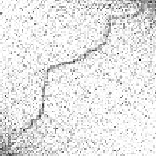
\includegraphics[width=120mm]{../img/walker.pdf}
\caption{A histogram of a generated matrix avoiding pattern~$P_1$.}
\label{walker}
\end{figure}

\begin{figure}[h!]
\centering
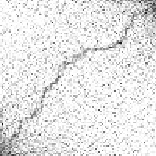
\includegraphics[width=120mm]{../img/walker2.pdf}
\caption{A histogram of a generated matrix avoiding pattern~$P_2$ using a different random seed than the previous picture.}
\label{walker2}
\end{figure}

\chapter*{Conclusion}
\addcontentsline{toc}{chapter}{Conclusion}
We have seen, how to use Markov chain Monte Carlo method to approximate a random matrix of given size avoiding a given set of forbidden patterns. We have used a heavily improved brute force algorithm to test avoidance of a general pattern and a simple dynamic programming algorithm for testing avoidance of a pattern, where all one-entries are contained on a walk in the pattern. To even more improve performance of the program, we have used parallel computing in the layer of the MCMC process.

The question is, whether we can do better? We probably cannot asymptotically improve the walking pattern avoidance algorithm (more in Chapter \ref{chap:walking}), because it is already linear in the number of elements of the matrix and computes only those elements that have changed. On the other hand, the algorithm is only useful for a small portion of all possible patterns. A natural question is, whether we can do as good for other classes of matrices?

In Section \ref{wholestructure}, we mentioned an alternative algorithm for testing avoidance of general patterns. Although it is probably not a very good algorithm for big matrices, because it needs to store all possible partial mappings, it may still turn out to be much better for smaller matrices, which are still big enough to see a structure in them, than the implemented algorithm is.

To use parallelism, we decided to use the MCMC layer of the program. There were several reasons to do so. First of all, it is not dependent on the avoidance pattern algorithm; therefore, if someone comes with a better one, it can still use the parallel version of MCMC. Secondly, when the matrix gets complex enough, the probability a change of one element is going to be successful is very small; thus, we have chosen to iterate through unsuccessful changes faster over the possibility to test avoidance faster.

A different approach would be to make avoidance testing parallel. In walking pattern, we could recompute multiple elements of the same diagonal at once, because they do not influence each other. In the algorithm for general patterns, we could generate new partial mappings in parallel, since they are independent. The only problem there is deciding whether two mappings are equivalent.

%%% Bibliography
%%% Bibliography (literature used as a source)
%%%
%%% We employ bibTeX to construct the bibliography. It processes
%%% citations in the text (e.g., the \cite{...} macro) and looks up
%%% relevant entries in the bibliography.bib file.
%%%
%%% The \bibliographystyle command selects, which style will be used
%%% for references from the text. The argument in curly brackets is
%%% the name of the corresponding style file (*.bst). Both styles
%%% mentioned in this template are included in LaTeX distributions.

\bibliographystyle{plainnat}    %% Author (year)
% \bibliographystyle{unsrt}     %% [number]

\renewcommand{\bibname}{Bibliography}

%%% Generate the bibliography. Beware that if you cited no works,
%%% the empty list will be omitted completely.

\bibliography{bibliography}

%%% If case you prefer to write the bibliography manually (without bibTeX),
%%% you can use the following. Please follow the ISO 690 standard and
%%% citation conventions of your field of research.

% \begin{thebibliography}{99}
%
% \bibitem{lamport94}
%   {\sc Lamport,} Leslie.
%   \emph{\LaTeX: A Document Preparation System}.
%   2nd edition.
%   Massachusetts: Addison Wesley, 1994.
%   ISBN 0-201-52983-1.
%
% \end{thebibliography}


%%% Figures used in the thesis (consider if this is needed)
\listoffigures

%%% Tables used in the thesis (consider if this is needed)
%%% In mathematical theses, it could be better to move the list of tables to the beginning of the thesis.
\listoftables

%%% Abbreviations used in the thesis, if any, including their explanation
%%% In mathematical theses, it could be better to move the list of abbreviations to the beginning of the thesis.
%%%\chapwithtoc{List of Abbreviations}

%%% Attachments to the bachelor thesis, if any. Each attachment must be
%%% referred to at least once from the text of the thesis. Attachments
%%% are numbered.
%%%
%%% The printed version should preferably contain attachments, which can be
%%% read (additional tables and charts, supplementary text, examples of
%%% program output, etc.). The electronic version is more suited for attachments
%%% which will likely be used in an electronic form rather than read (program
%%% source code, data files, interactive charts, etc.). Electronic attachments
%%% should be uploaded to SIS and optionally also included in the thesis on a~CD/DVD.
\chapwithtoc{Attachments}

\openright
\end{document}
